\documentclass[landscape]{foils} 
\newif\ifpdf
\ifx\pdfoutput\undefined
\pdffalse % we are not running PDFLaTeX
\else
\pdfoutput=1 % we are running PDFLaTeX
\pdftrue
\fi

\ifpdf
\usepackage[pdftex]{graphicx}
\else
\usepackage{graphicx}
\fi

\ifpdf
\DeclareGraphicsExtensions{.pdf, .jpg, .tif, .png}
\else
\DeclareGraphicsExtensions{.eps, .jpg}
\fi

%\usepackage{pslatex}
\usepackage{tabularx,dcolumn, graphicx, amsfonts,amsmath}  
\usepackage[sectionbib]{natbib}
\bibliographystyle{apalike}
\usepackage{picinpar}
\usepackage{multirow}
\usepackage{rotating}
\usepackage{paralist} %compactenum
\setlength{\voffset}{-0.5in}
%\setlength{\hoffset}{-0.5in}
%\setlength{\textwidth}{10.5in}
\setlength{\textheight}{7in}
\setlength{\parindent}{0pt}
%\pagestyle{empty}
%\renewcommand{\baselinestretch}{2.0}
\DeclareMathSymbol{\expect}{\mathalpha}{AMSb}{'105}
\def\p{\rm p}
\def\pp{\rm P}
% this are commands that come with the color package
\usepackage{color}
\usepackage{fancyhdr}


\pagestyle{empty}
%define colors
\definecolor{mediumblue}{rgb}{0.0509,0.35,0.568}
\definecolor{blue}{rgb}{0.0109,0.15,0.468}
\definecolor{black}{rgb}{0.04,0.06,0.2}
\definecolor{darkblue}{rgb}{0.03,0.1,0.2}
\definecolor{darkgreen}{rgb}{0.03,0.5,0.2}
\definecolor{lightblue}{rgb}{0.85,0.9333,0.95}
\definecolor{lightblue2}{rgb}{0.270588, 0.45098, 0.701961}
\definecolor{white}{rgb}{1.0,1.0,1.0}
\definecolor{yellow}{rgb}{0.961,0.972,0.047}
\definecolor{red}{rgb}{0.9,0.1,0.1}
\definecolor{orange}{rgb}{1.0,0.4,0.0}
\definecolor{grey}{rgb}{0.5,0.5,0.5}
\definecolor{violet}{rgb}{0.619608, 0.286275, 0.631373}
\definecolor{mybackgroundcolor}{rgb}{1.0,1.0,1.0}

%\definecolor{light}{rgb}{.5,0.5,0.0}
\definecolor{light}{rgb}{.3,0.3,0.3}

% sets backgroundcolor for whole document 
\pagecolor{mybackgroundcolor}
% sets text color
%\color{black}
% see below for an example how to change just a few words
% using \textcolor{color}{text}

\font \courier=pcrb scaled 2000
\newcommand{\notetoself}[1]{{\textsf{\textsc{\color{red} #1}}}\\}

\newcommand{\answer}[1]{{\sf \color{red} #1}}

\usepackage{pdfpages}

\newcommand{\section}{\secdef \newsection\newsection}
%\renewcommand{\labelitemi}{\includegraphics[width=5mm]{images/bullet.pdf}}
\newcommand{\newsection}[1]{%
{
	\par\flushleft\large\sf\bfseries \vskip -2cm #1\\\rule[0.7\baselineskip]{\textwidth}{0.5mm}\par}}

\newcommand{\subsection}{\secdef \test\test}
\newcommand{\test}[1]{%
	{\par\flushleft\normalsize\sf\bfseries #1: }}
\newcommand{\M}{\mathcal{M}}
\newcommand{\prob}{{\rm Prob~}}
\def\showy#1{{\normalsize\sf\bfseries #1}}
\def\donotuse#1{}

\newcommand{\entrylabel}[1]{\mbox{#1}\hfil}
\newenvironment{entry}
	{\begin{list}{}%
		{\renewcommand{\makelabel}{\entrylabel}%
		\setlength{\labelwidth}{35pt}%
		\setlength{\leftmargin}{\labelwidth+\labelsep}%
	}%
	{\end{list}}}

\newcommand{\poltext}{{\copyright\ 2002--2010 by Paul O. Lewis -- Modified by  Mark Holder with permission from Paul Lewis}}

\newcommand{\pol}{{\footnotesize \poltext}}
\newcommand{\myBackground}{\begin{picture}(0,0)(0,0)  \put(-40,-70){\makebox(0,0)[l]{\includegraphics[width=33cm]{images/baby_blue.jpg}}} \end{picture}}
\newcommand{\myFooter}{}
%\begin{picture}(0,0)(0,0)
%	\put(0,-185){\pol}
%\end{picture}}
\newcommand{\myNewSlide}{\newpage\myFooter} % \myBackground}

\usepackage{bm}
\usepackage{mathrsfs}
\usepackage{url}
\usepackage{hyperref}
\hypersetup{backref,  linkcolor=blue, citecolor=black, colorlinks=true, hyperindex=true}

\usepackage{pdfpages}
\usepackage{bm}

\begin{document}

\myNewSlide
\huge 
{\begin{center}Testing phylogenetic hypotheses\end{center}}
\vskip 3cm
\large Woods Hole Workshop on Molecular Evolution, 2013\par 
\vskip 3cm
\normalsize
\normalsize
Mark T. Holder\\
University of Kansas\par 
\vskip 1cm
Thanks to Paul Lewis, Joe Felsenstein, and Peter Beerli for slides.

\myNewSlide
\section*{Reasons phylogenetic inference might be wrong}
\Large
\begin{compactenum}
	\item {\em Systematic error} -- Our inference method might not be sophisticated enough
	\item \underline{{\em Random error}} -- We might not have enough data --  we are misled by sampling error.
\end{compactenum}

(or it could be some combination of these).

{Focus of this evening: {\bf How confident can we be in the trees/splits inferred by ML?}}

\myNewSlide
\begin{compactenum}
	\item Bootstrapping
	\item Putting $P$-values on trees:
	\begin{compactitem}
		\item KH Test, SH Test
		\item parametric bootstrapping,
		\item aLRT, aBayes,
		\item 1 - BP,
		\item AU and \citet{EfronHH1996} correction
		\item aBP
	\end{compactitem}
	\item Cartoon time! ({\small warning: ``cartoon time'' will not actually be fun})
\end{compactenum}

\myNewSlide
\section*{Some resources related to this talk}
A \href{http://www.zotero.org/groups/confidence_statements_on_phylogenies}{Zotero Group} of papers related to topology testing on trees.

A \url{http://phylo.bio.ku.edu/woodshole/index.html} has the beginnings of an annotated bibliography and some other notes.

The source for all the documents for my talk are at:\\ {\normalsize \url{https://github.com/mtholder/TreeTopoTestingTalks} }\\
{\normalsize \url{https://github.com/mtholder/treeTestingDemo}}


\myNewSlide
\begin{picture}(0,0)(0,0)
	  \put(-60,-280){\makebox(0,0)[l]{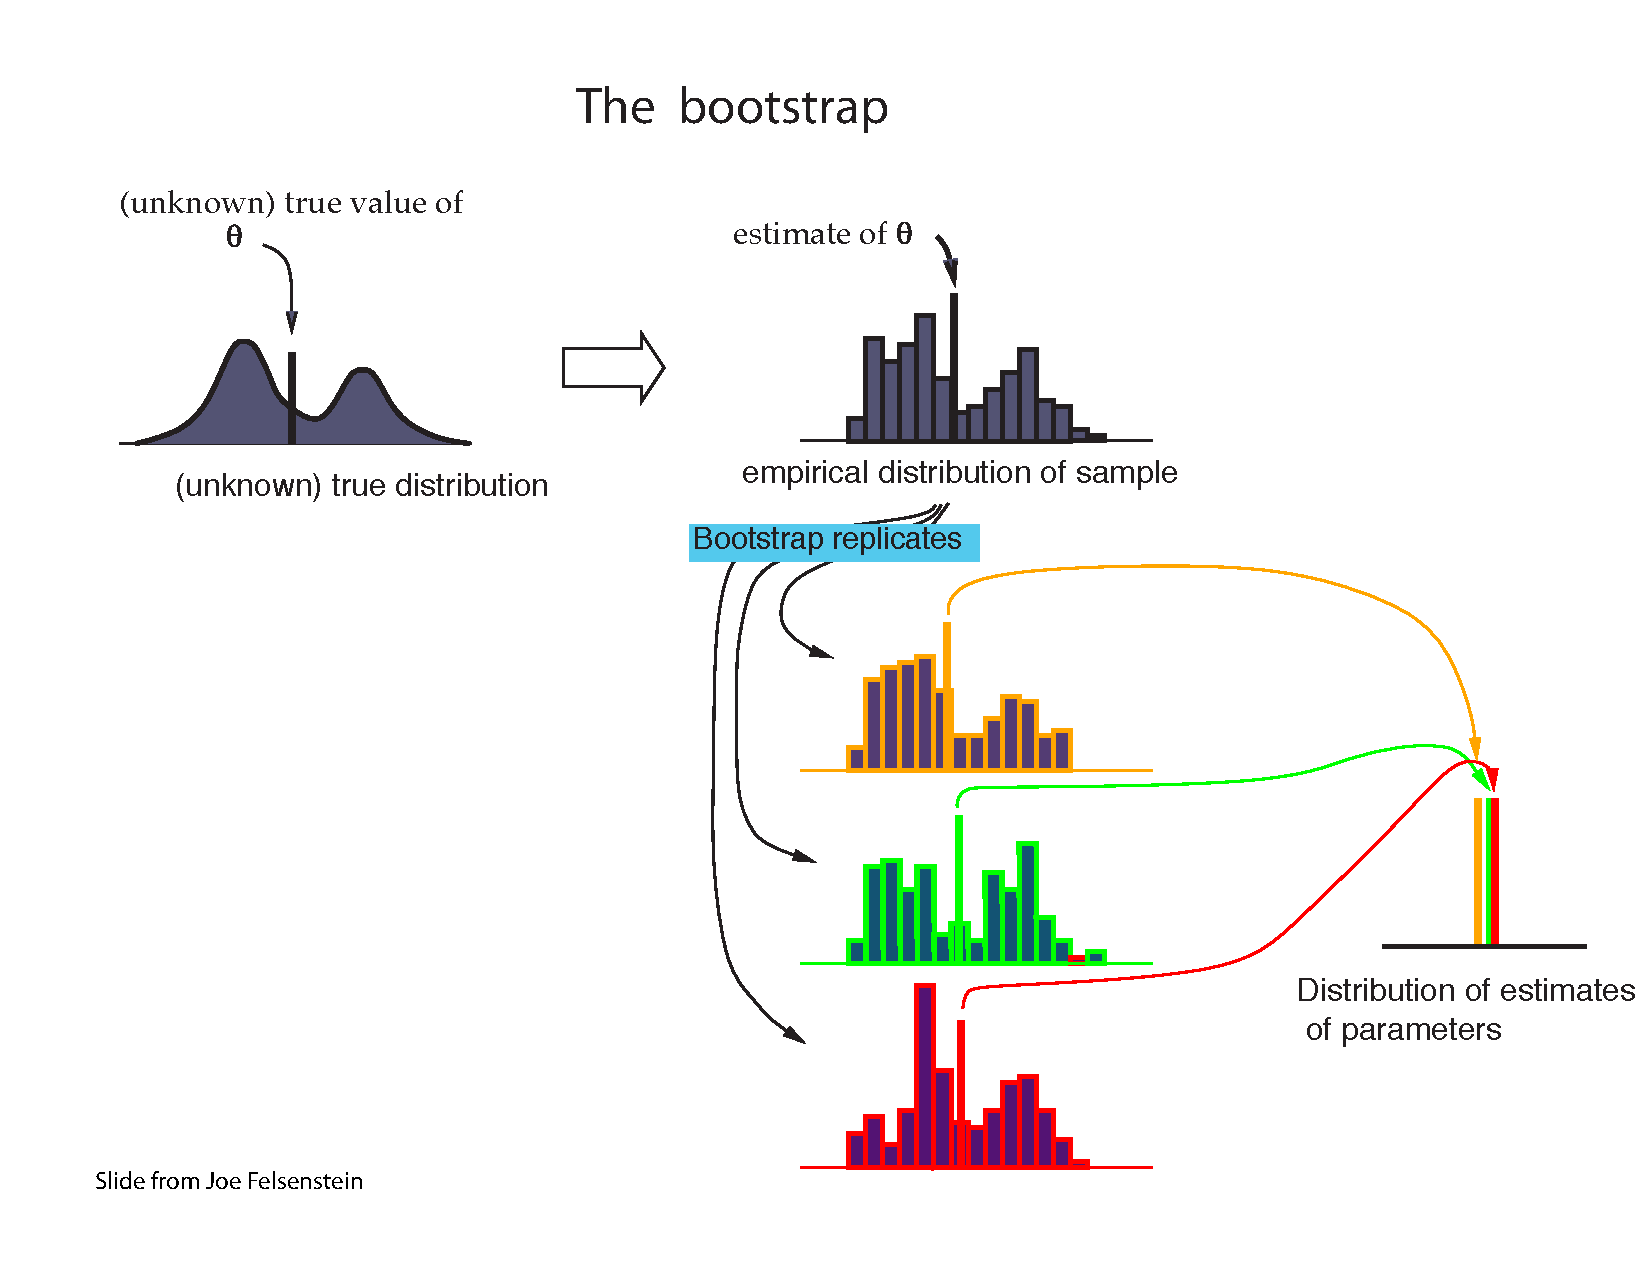
\includegraphics[scale=1.2]{../newimages/JoeFelsBootFig1.pdf}}}
	  \put(0,-716){\makebox(0,0)[l]{
\includegraphics[scale=2]{../newimages/whitepage.pdf}}}
\end{picture}

\myNewSlide
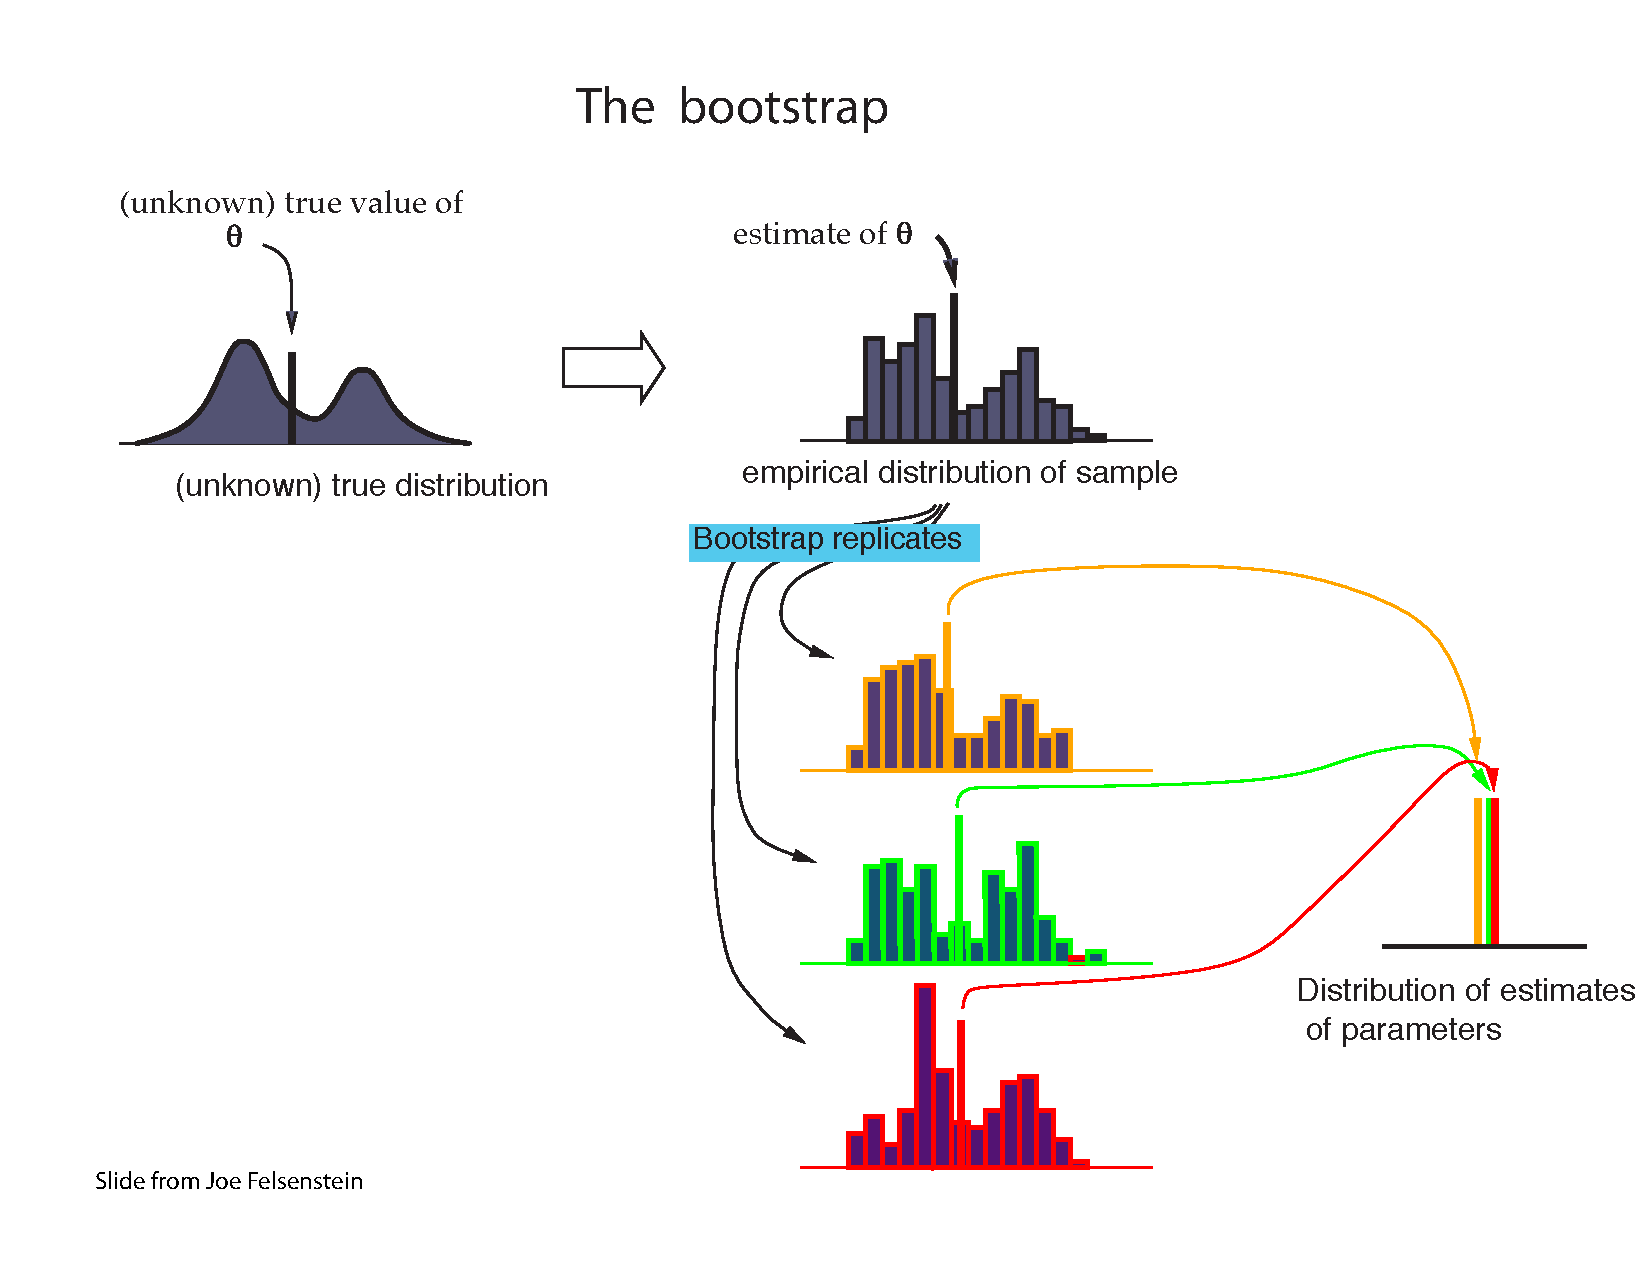
\includepdf[pages={1}]{../newimages/JoeFelsBootFig1.pdf} 

\myNewSlide
\begin{picture}(0,0)(0,0)
	  \put(-70,-316){\makebox(0,0)[l]{
\includegraphics[scale=2]{../newimages/greypage.pdf}}}
	  \put(-40,-200){\makebox(0,0)[l]{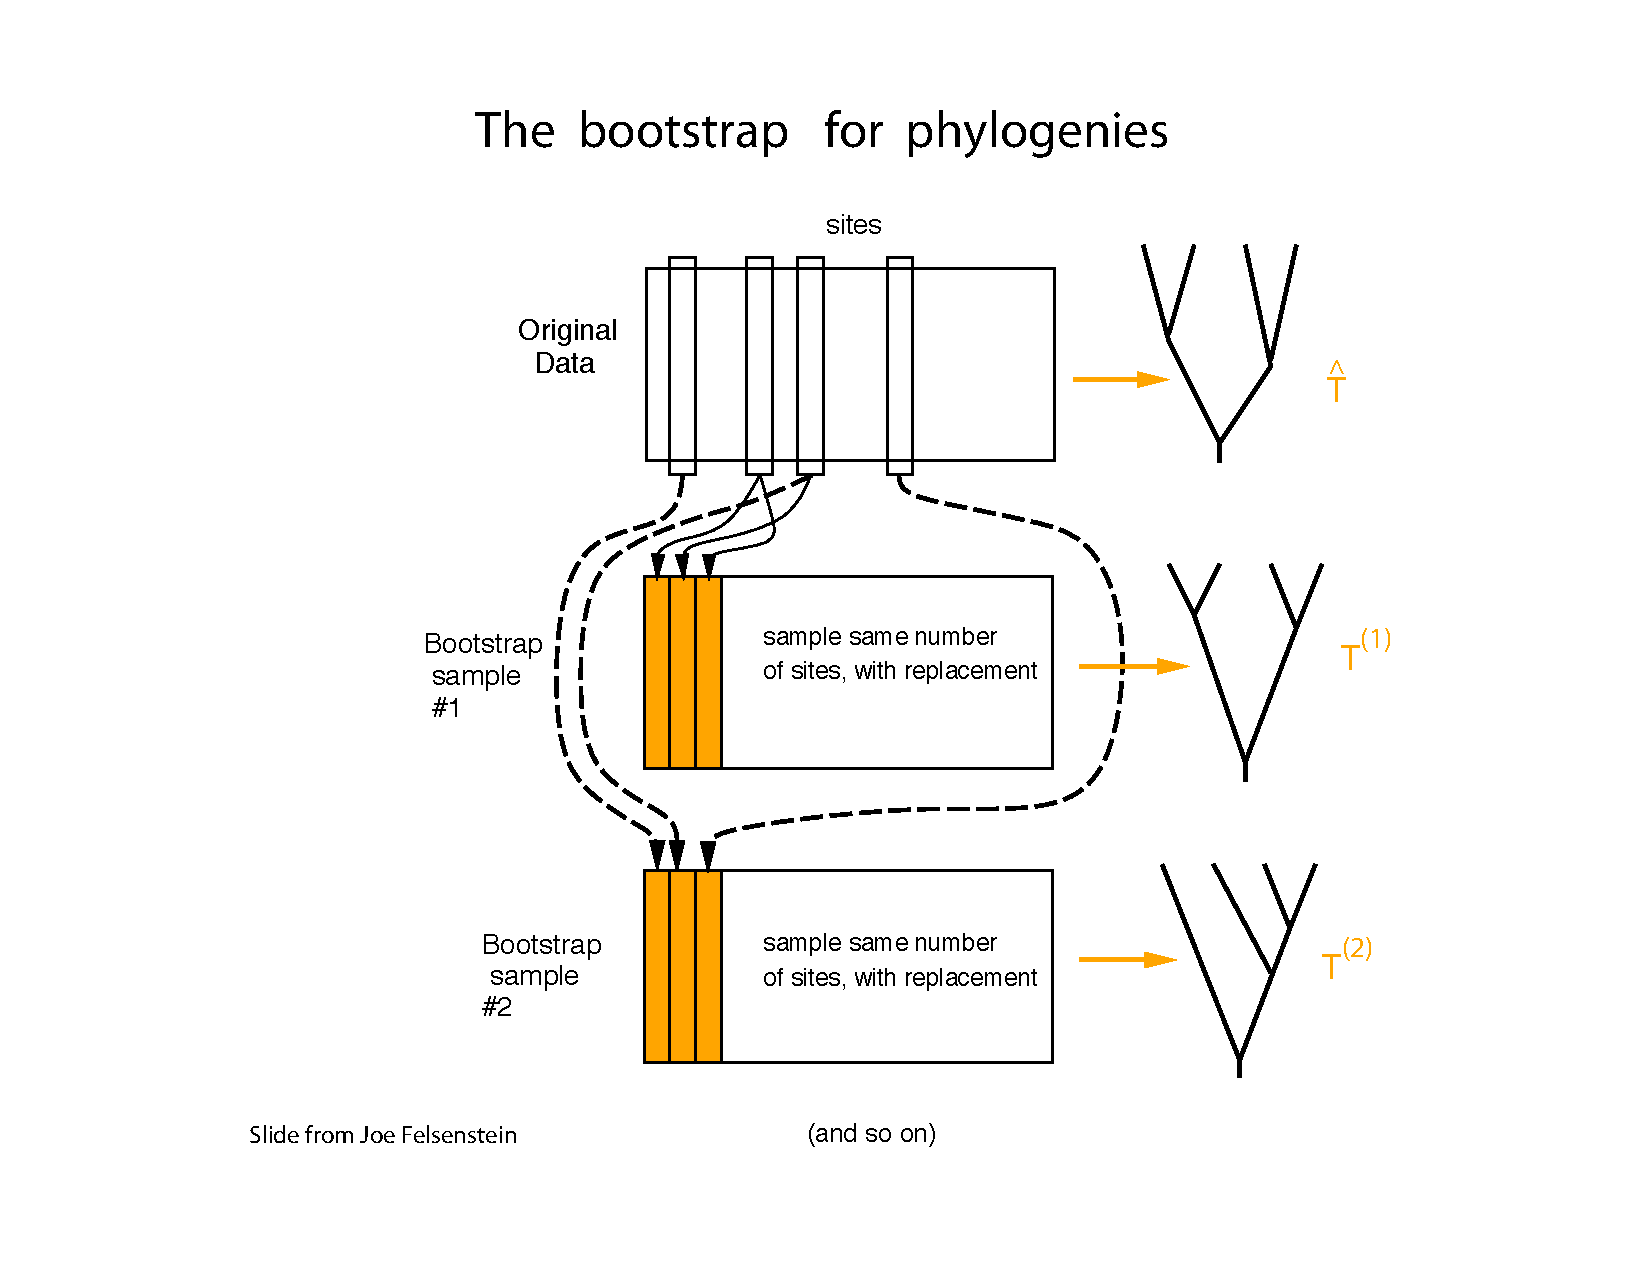
\includegraphics[scale=1.0]{../newimages/JoeFelsBootFig2.pdf}}}
\end{picture}

\myNewSlide
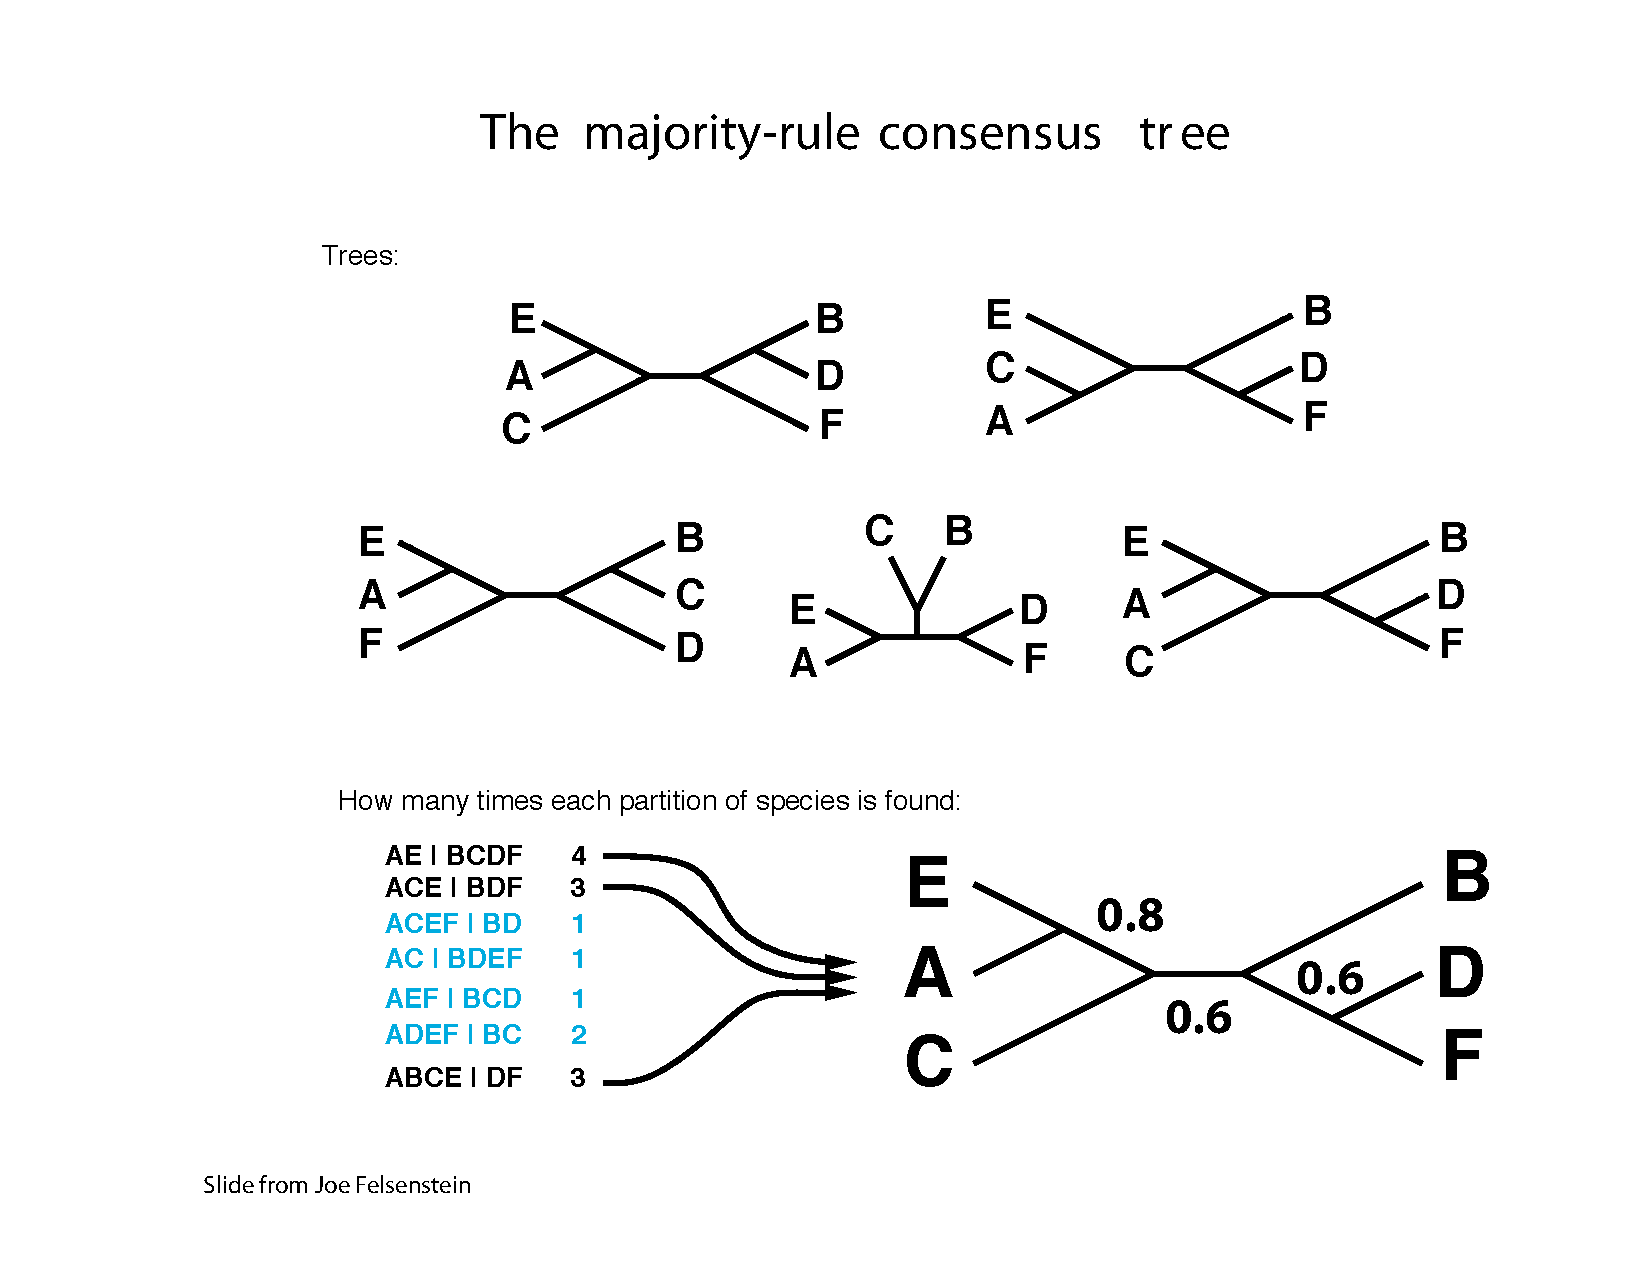
\includepdf[pages={1}]{../newimages/JoeFelsBootFig3.pdf} 

\myNewSlide
\begin{picture}(0,0)(0,0)
	  \put(0,-180){\makebox(0,0)[l]{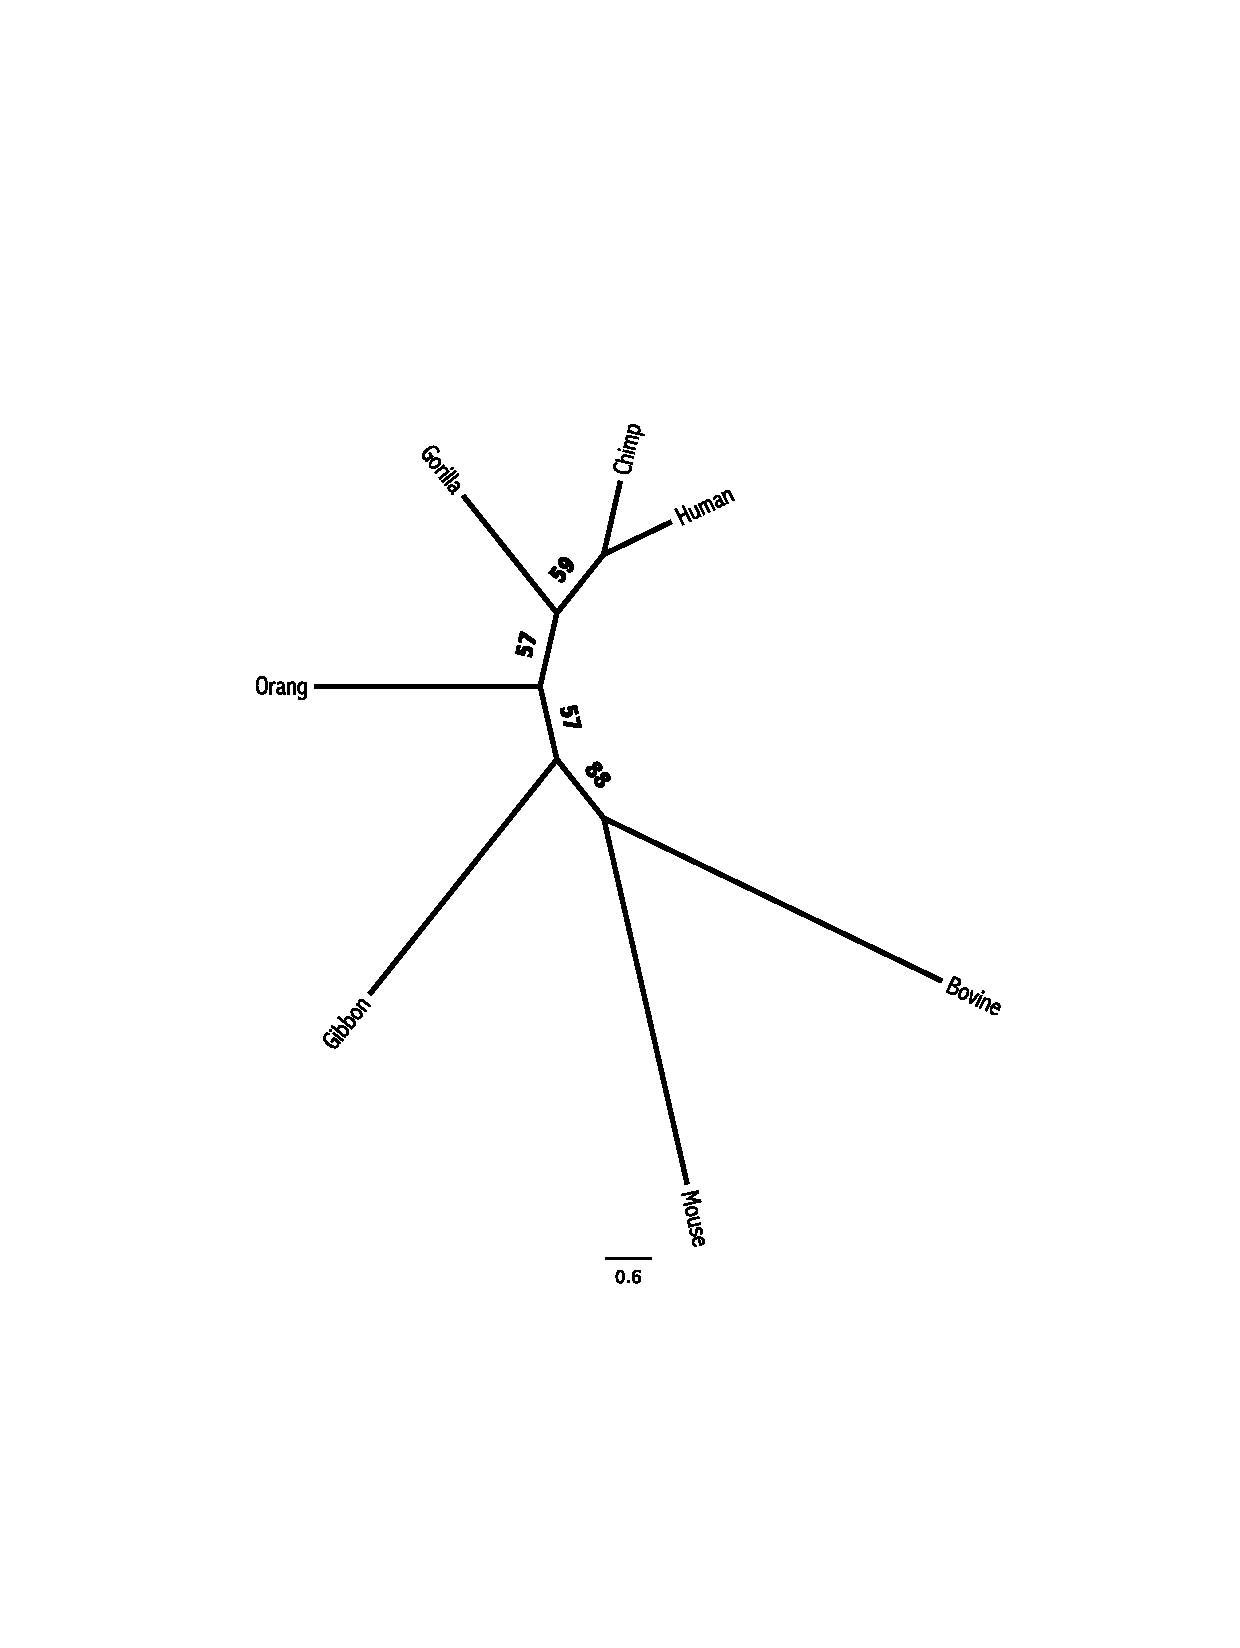
\includegraphics[scale=1.2]{../newimages/hasegawaBootFigTree.pdf}}}
	  \put(0,-350){\small From Hasegawa's analysis of 232 sites D-loop}
\end{picture}

\myNewSlide
\section*{Bootstrapping for branch support}
\large
\begin{itemize}
	\item Typically a few hundred bootstrap, pseudoreplicate datasets are produced.
	\item Less thorough searching is faster, but will usually artificially lower bootstrap proportions (BP). However, \citet{AnisimovaGDDG2011} report that RAxML's rapid bootstrap algorithm may inflate BP.
	\item ``Rogue'' taxa can lower support for many splits -- you do not have to use the majority-rule consensus tree to summarize bootstrap confidence statements.
\end{itemize}



\myNewSlide
\section*{Frequentist hypothesis testing: coin flipping example}
$N=100$ and $h=60$\\
Can we reject the fair coin hypothesis? $H_0:\Pr(\mbox{heads}) = 0.5$

The ``recipe'' is:
\begin{compactenum}
	\item Formulate null ($H_0$) and alternative ($H_A$) hypotheses.
	\item Choose an acceptable Type-I error rate (significance level)
	\item Choose a test statistic: $f_H$= fraction of heads in sample. $f_H=0.6$
	\item Characterize the null distribution of the test statistic 
	\item Calculate the $P$-value: The probability of a test statistic value more extreme than $f_H$ arising {\em even if $H_0$  is true}.
	\item Reject $H_0$ if $P$-value is $\leq$ your Type I error rate.
\end{compactenum}

\myNewSlide
\begin{picture}(500,0)(0,0)
	  \put(0,-190){\makebox(0,0)[l]{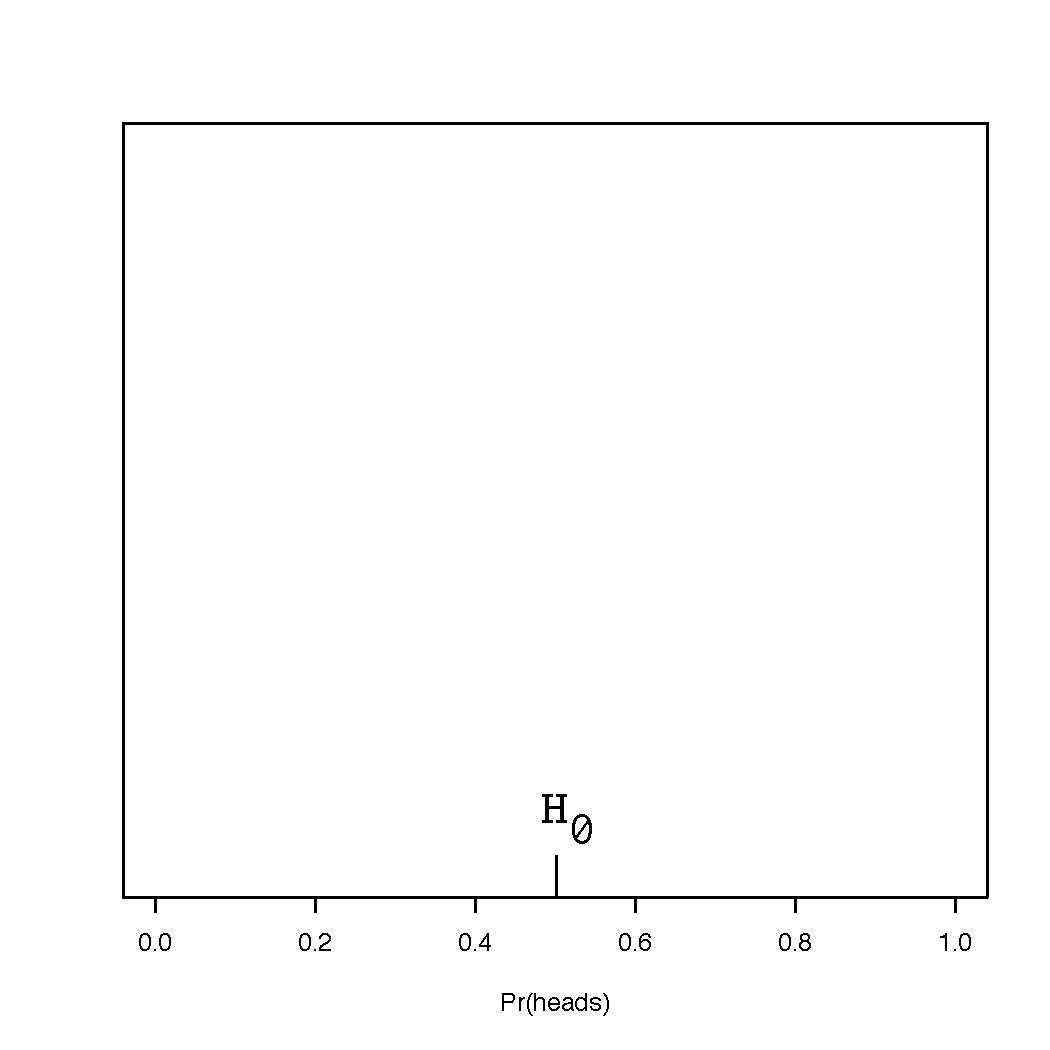
\includegraphics[scale=1.0]{../newimages/coin_axes.pdf}}}
\end{picture}

\myNewSlide
\begin{picture}(500,0)(0,0)
	  \put(0,-190){\makebox(0,0)[l]{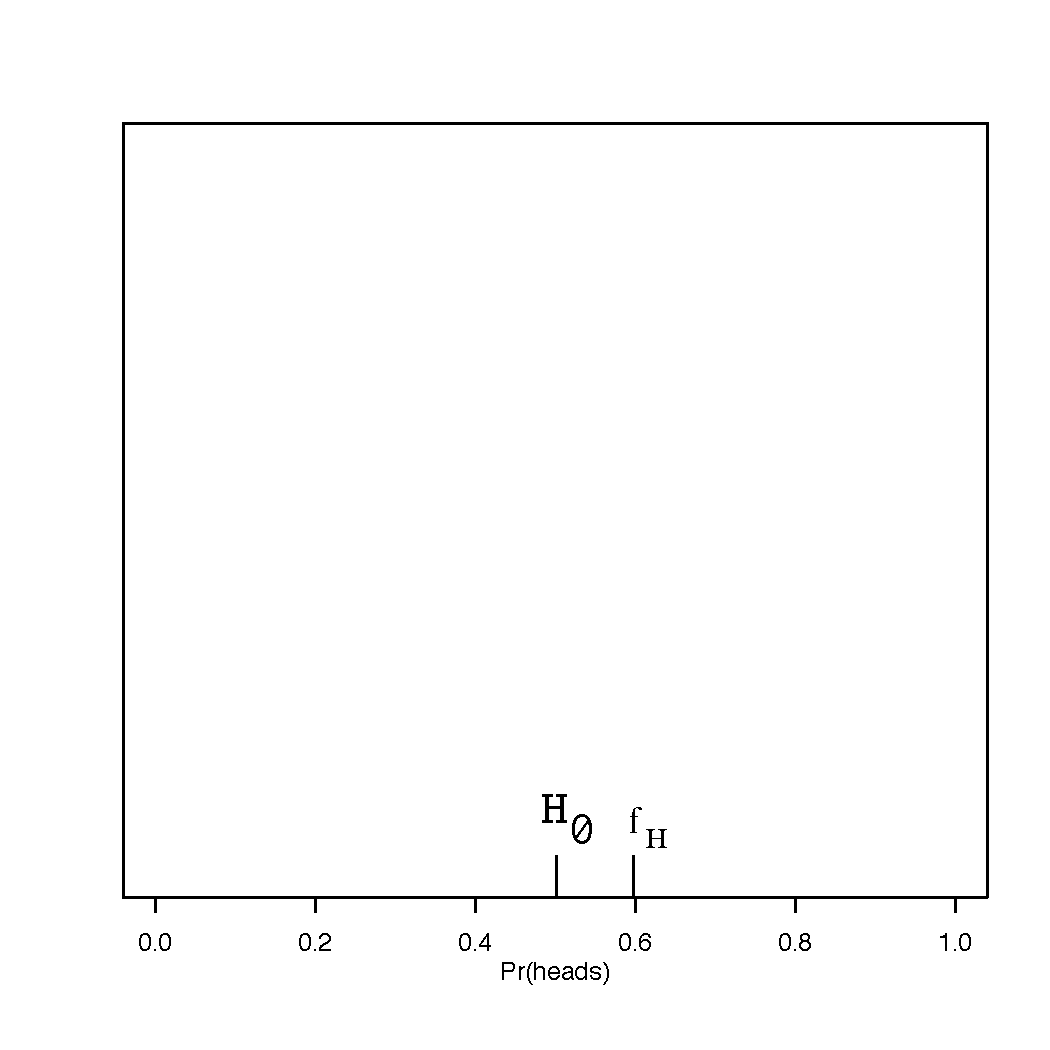
\includegraphics[scale=1.0]{../newimages/coin_axes_data.pdf}}}
\end{picture}

\myNewSlide
\section*{Null distribution}
\begin{picture}(500,0)(0,0)
	  \put(0,-190){\makebox(0,0)[l]{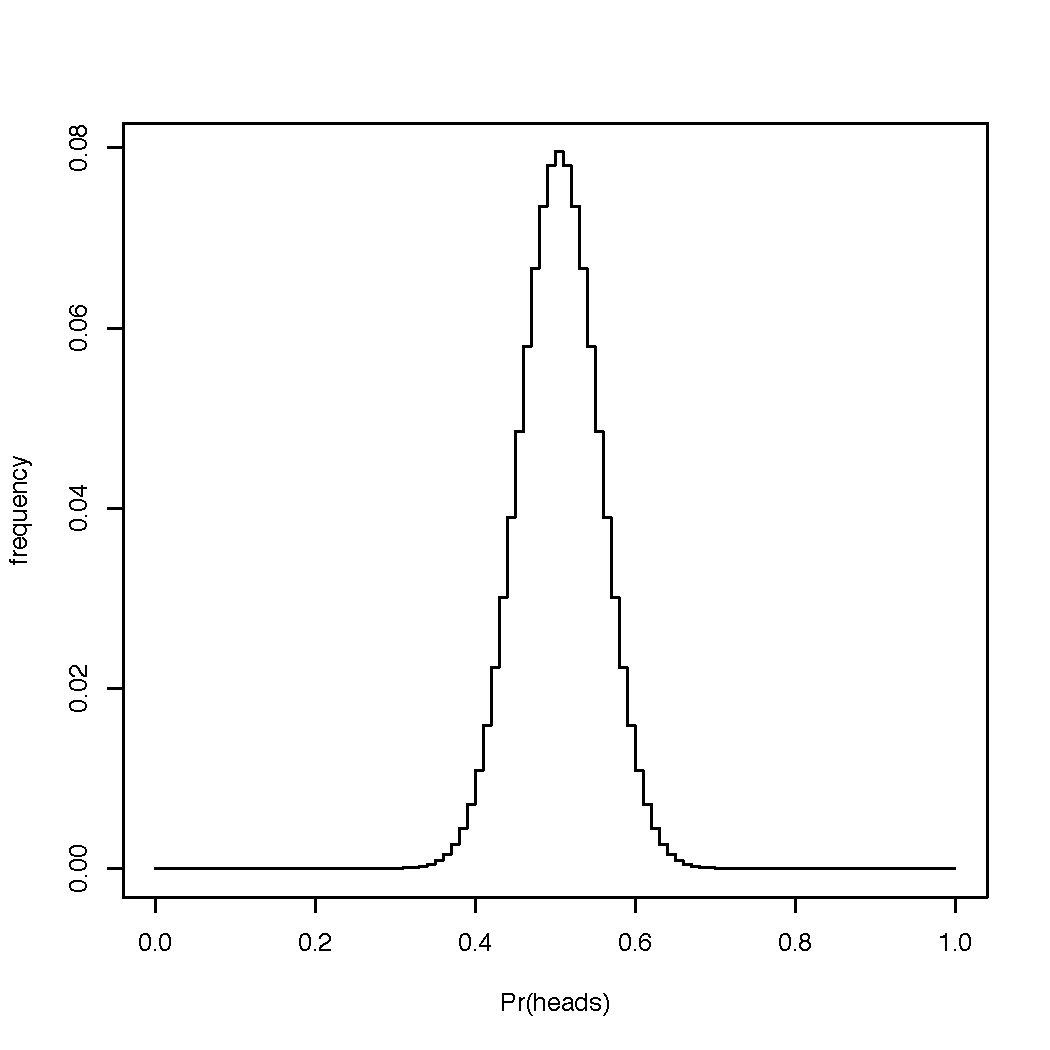
\includegraphics[scale=1.0]{../newimages/coin_wo_tails.pdf}}}
\end{picture}

\myNewSlide
\begin{picture}(500,0)(0,0)
	  \put(0,-190){\makebox(0,0)[l]{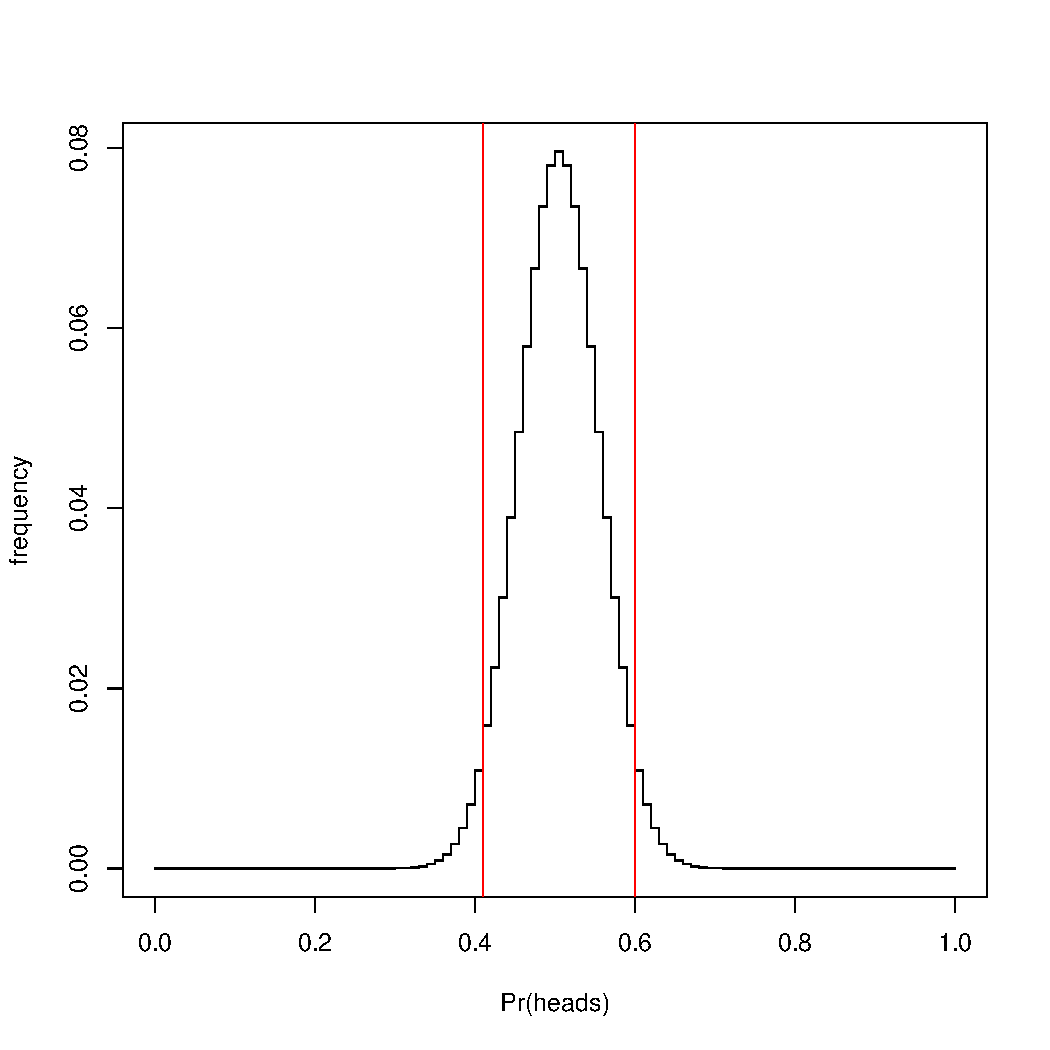
\includegraphics[scale=1.0]{../newimages/coin_w_tails.pdf}}}
	  \put(0,-450){$P$-value $\approx$ 0.058}
\end{picture}

\myNewSlide
Making similar plots for tree inference is hard.

\begin{itemize}
	\item Our parameter space is trees and branch lengths.
	\item Our data is a matrix of characters.
	\item It is hard to put these objects on the same plot.
	\item We will see later (during ``cartoon time''), that we {\em can} visualize them both in a parameter space that describes the frequency of different data patterns.
\end{itemize}




\myNewSlide
\section*{The simplest phylogenetic test would compare two trees}
\Large
Null: If we had no sampling error (infinite data) $T_1$ and $T_2$ would explain the data equally well. 

Test Statistic: $$\delta(T_1,T_2 \mid X) = 2\left[\ln L(T_1 \mid X) - \ln L(T_2 \mid X)\right]$$

Expectation under null: $$\mathbb{E}_{H_0}\left[\delta(T_1,T_2 \mid X)\right] = 0$$


\myNewSlide
\begin{picture}(500,0)(-20,-50)
	  \put(20,-20){\small Using 3000 sites of mtDNA sequence for 5 primates}
	  \put(20,-60){\normalsize $T_1$ is ((chimp, gorilla), human)}
	  \put(50,-200){\makebox(0,-190)[l]{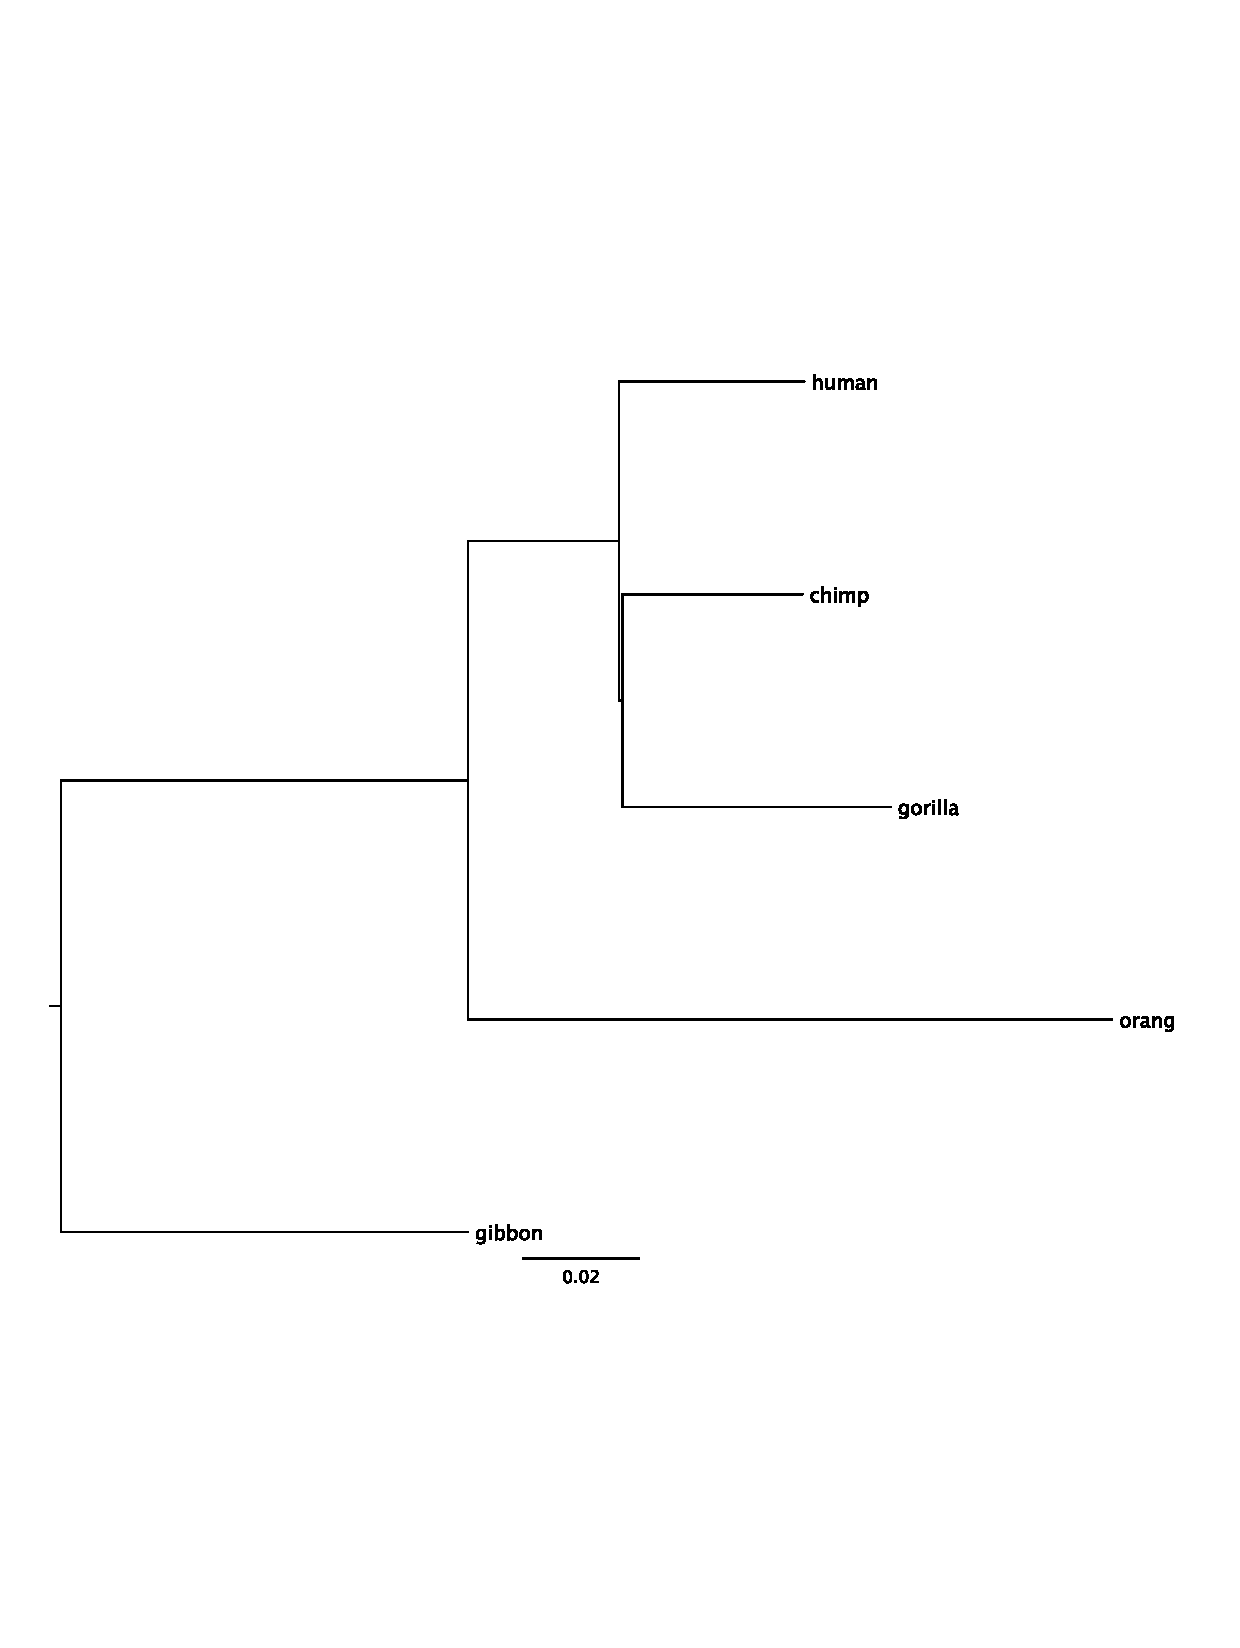
\includegraphics[scale=1.0]{../scripts/mtdna/chimpGorilla3000sites.pdf}}}
\end{picture}

\myNewSlide
\begin{picture}(500,0)(-20,-50)
	  \put(20,-20){\small Using 3000 sites of mtDNA sequence for 5 primates}
	  \put(20,-60){\normalsize $T_2$ is ((chimp, human), gorilla)}
	  \put(50,-200){\makebox(0,-190)[l]{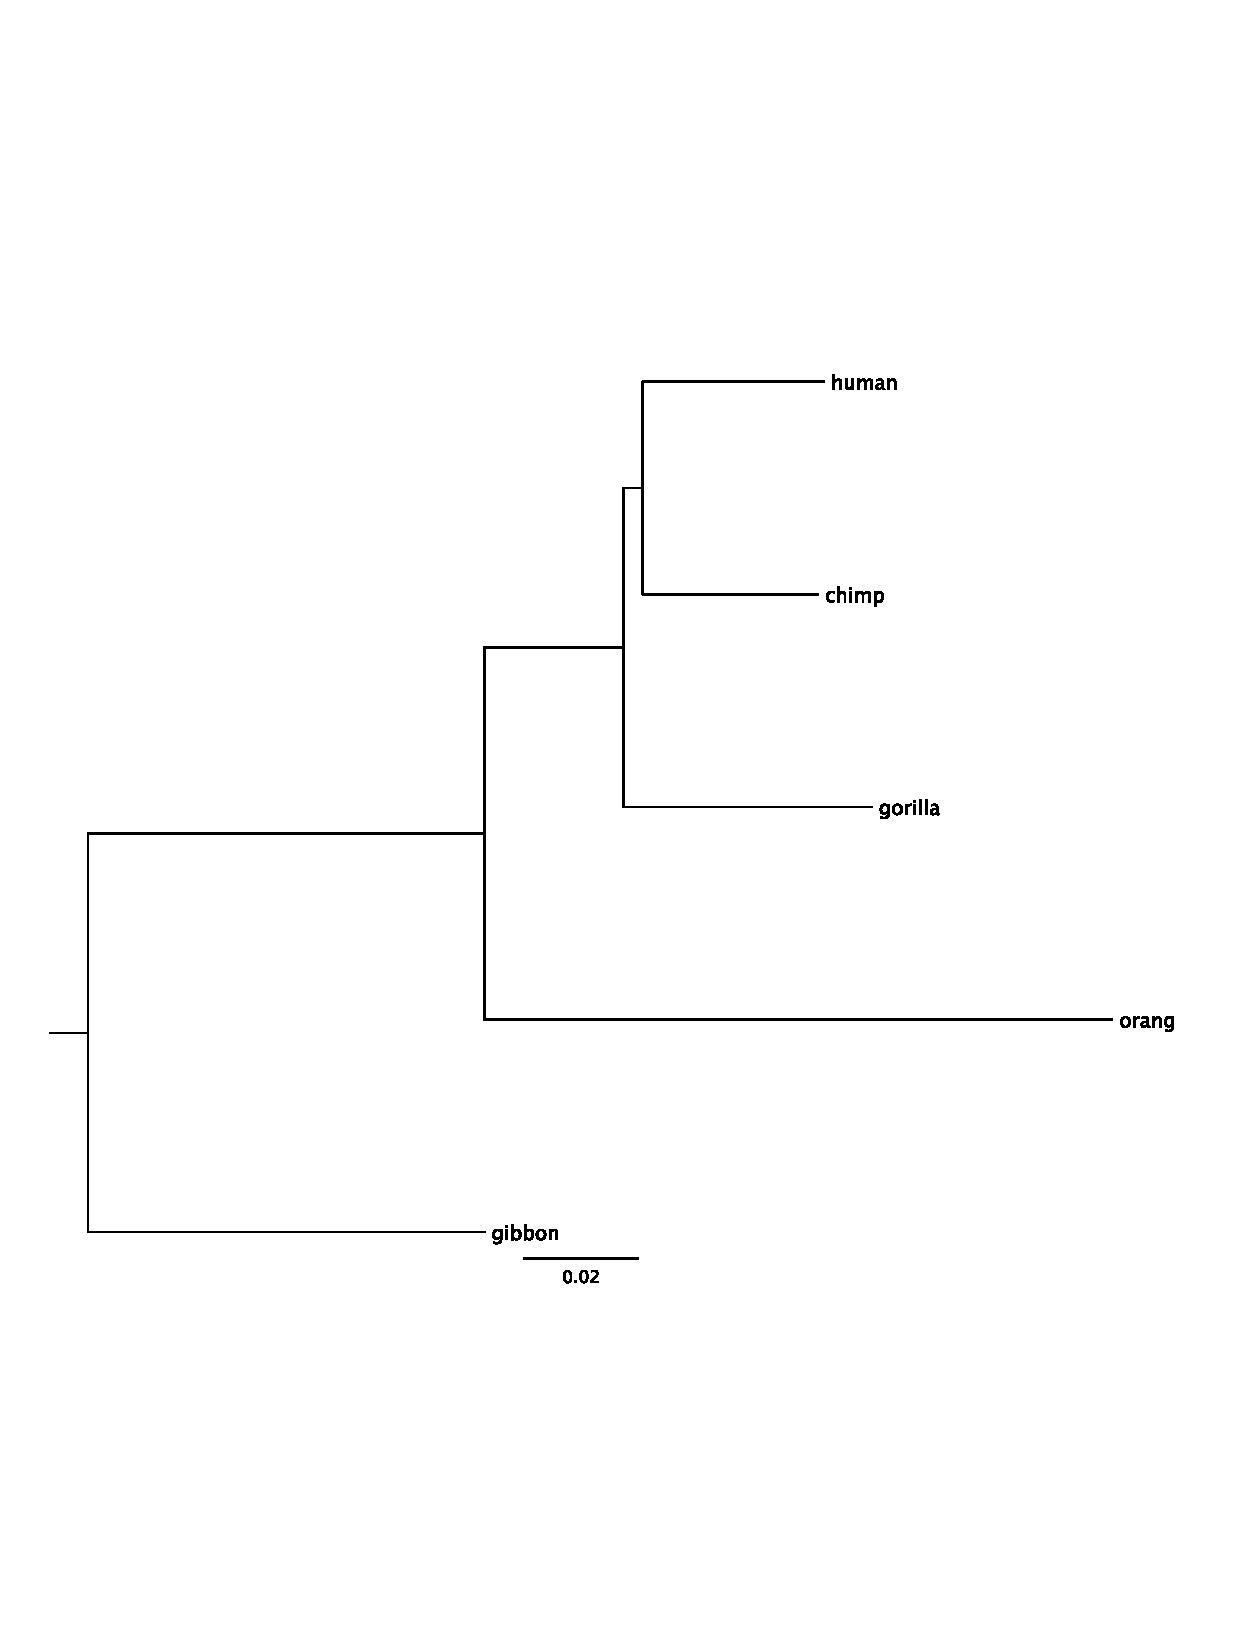
\includegraphics[scale=1.0]{../scripts/mtdna/humanChimp3000SitesTree.pdf}}}
\end{picture}

\myNewSlide
\begin{picture}(500,0)(-20,-50)
	  \put(20,-20){\small Using 3000 sites of mtDNA sequence for 5 primates}
	  \put(20,-60){\normalsize $T_1$ is ((chimp, gorilla), human)   \hskip2cm $\ln L(T_1 \mid X) = -7363.296$}
	  \put(20,-100){\normalsize $T_2$ is ((chimp, human), gorilla)  \hskip2cm $\ln L(T_2 \mid X) = -7361.707$}
	  \put(-10,-385){\small$\delta(T_1,T_2 \mid X)=-3.18$}
	  \put(300,-385){\small$\mathbb{E}(\delta)$}
	  \put(50,-150){\makebox(0,-190)[l]{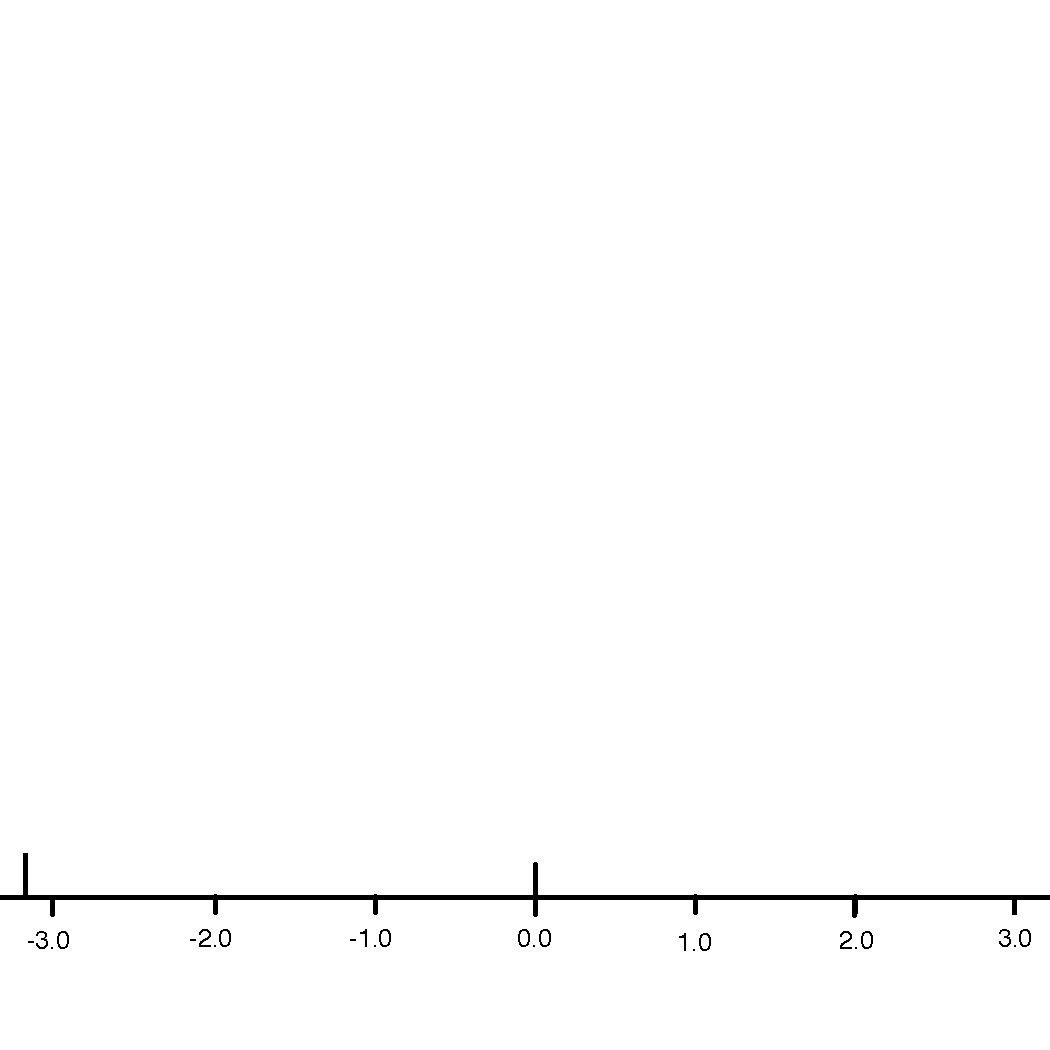
\includegraphics[scale=1.0]{../newimages/delta_axes.pdf}}}
	  \put(220,-480){$\delta(T_1,T_2 \mid X) $}
\end{picture}




\myNewSlide

To get the $P$-value, we need to know the probability: $$\Pr\left(\big | \delta(T_1,T_2 \mid X)\big |  \geq 3.18  {\bm{\Big|}}  H_0\mbox{ is true}\right) $$
\begin{picture}(500,0)(-20,-50)
	  \put(-10,-235){\small$\delta(T_1,T_2 \mid X)=-3.18$}
	  \put(460,-235){\small$-\delta(T_1,T_2 \mid X)=3.18$}
	  \put(10,-270){\huge$\leftarrow$}
	  \put(570,-270){\huge$\rightarrow$}
	  \put(300,-235){\small$\mathbb{E}(\delta)$}
	  \put(50,-0){\makebox(0,-190)[l]{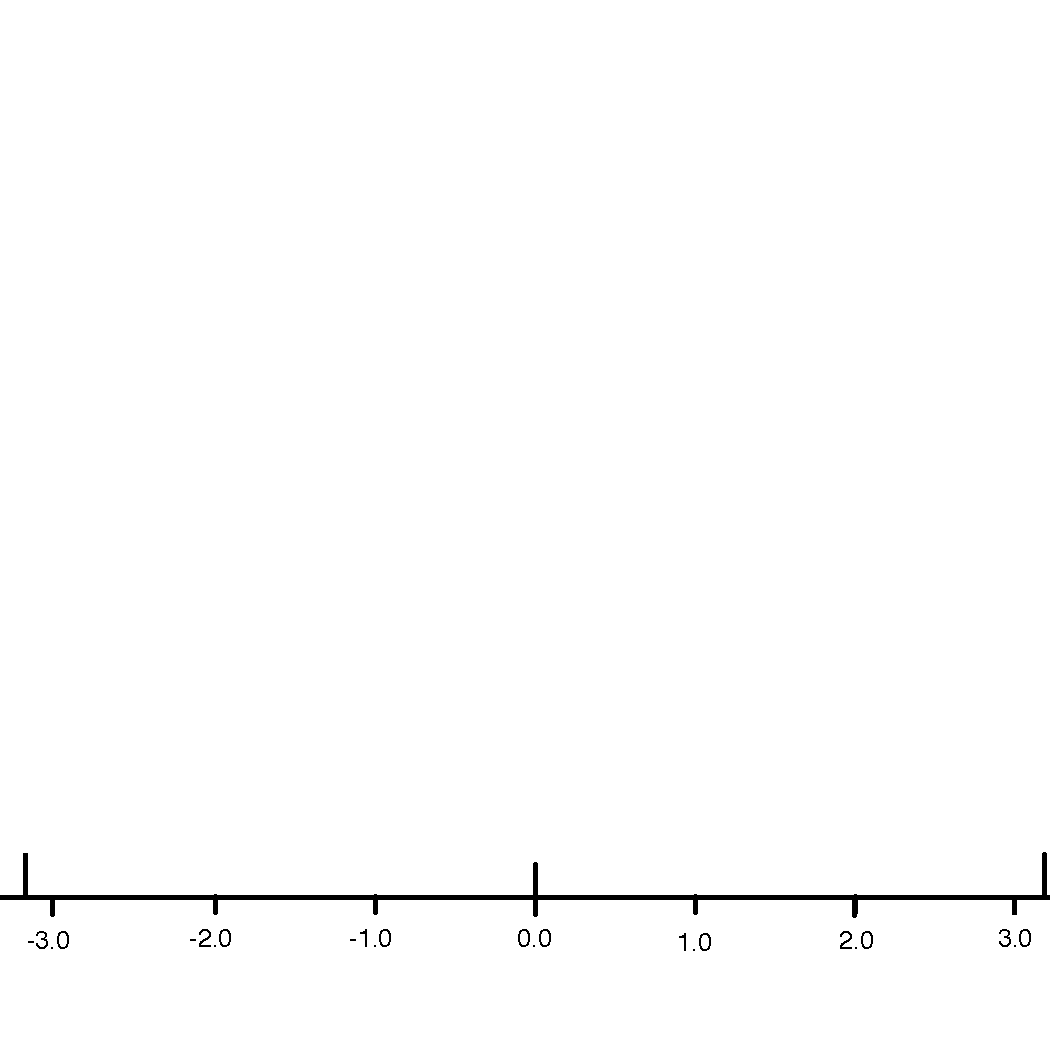
\includegraphics[scale=1.0]{../newimages/delta_axes_reflected.pdf}}}
	  \put(220,-330){$\delta(T_1,T_2 \mid X) $}
\end{picture}

\myNewSlide
\section*{KH Test}
\begin{compactenum}
	\item Examine the difference in $\ln L$ for each site: $\delta(T_1,T_2 \mid X_i)$ for site $i$.
	\item Note that the total difference is simply a sum:
		$$\delta(T_1,T_2 \mid X) = \sum_{i=1}^M\delta(T_1,T_2 \mid X_i)$$
	\item The variance of $\delta(T_1,T_2 \mid X)$ will be a function of the variance in ``site'' $\delta(T_1,T_2 \mid X_i)$ values.
\end{compactenum}



\myNewSlide
\begin{picture}(500,0)(0,0)
	  \put(0,10){\large $\delta(T_1,T_2 \mid X_i)$ for each site, $i$.}
	  \put(280,-35){\large $\vdots$}
	  \put(20,-250){\makebox(0,0)[l]{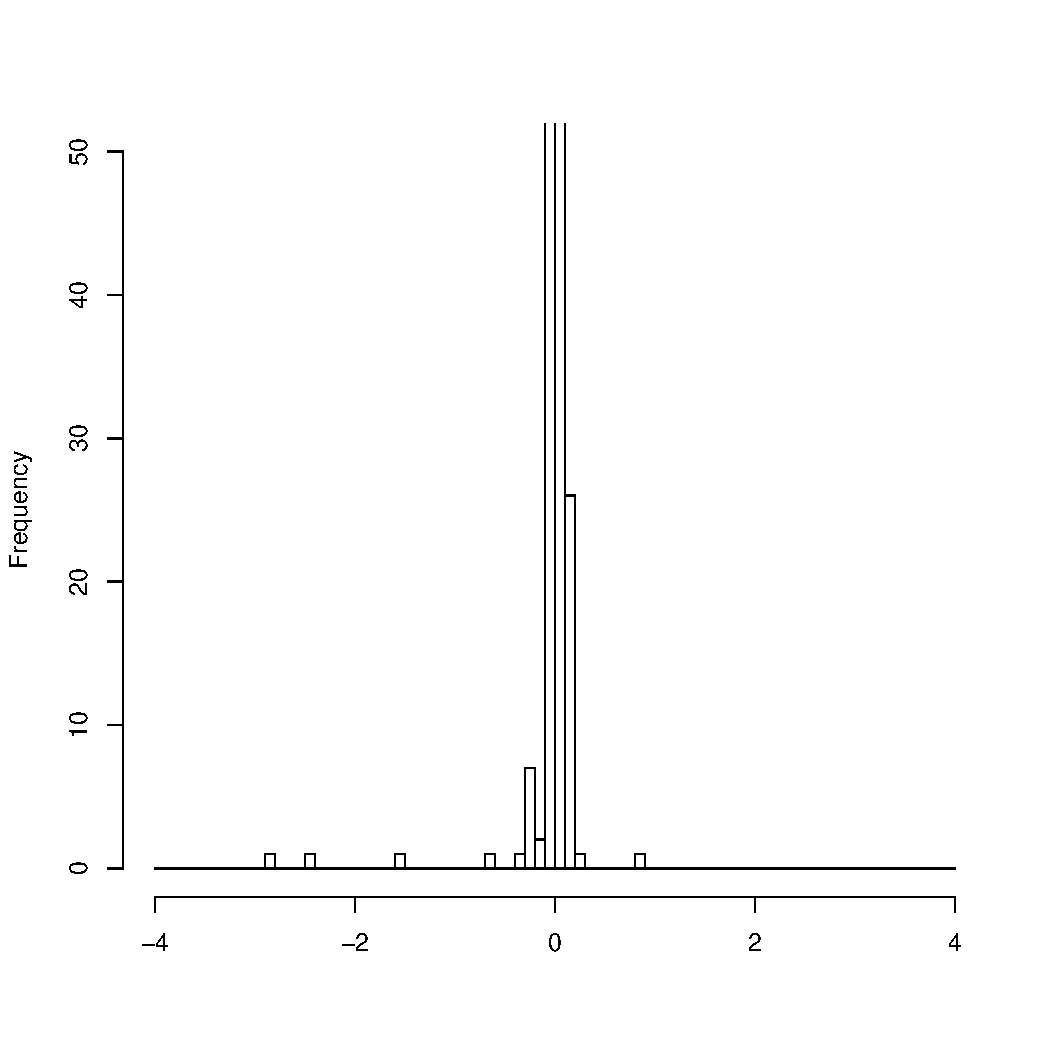
\includegraphics[scale=1.0]{../scripts/mtdna/d1-2hist.pdf}}}
	  \put(250,-490){\normalsize$\delta(T_1,T_2 \mid x_i)$}
\end{picture}


\myNewSlide
\section*{KH Test - the variance of $\delta(T_1,T_2 \mid X)$}
To approximate variance of $\delta(T_1,T_2 \mid X)$ under the null, we could:
\begin{compactenum}
	\item use assumptions of Normality (by appealing to the Central Limit Theorem). Or
	\item use bootstrapping to generate a cloud of pseudo-replicate $\delta(T_1,T_2 \mid X^{\ast})$ values, and look at their variance.
\end{compactenum}

\myNewSlide
\begin{picture}(500,0)(0,0)
	  \put(0,-10){\large $\delta$ for many (RELL) bootstrapped replicates of the data}
	  \put(20,-250){\makebox(0,0)[l]{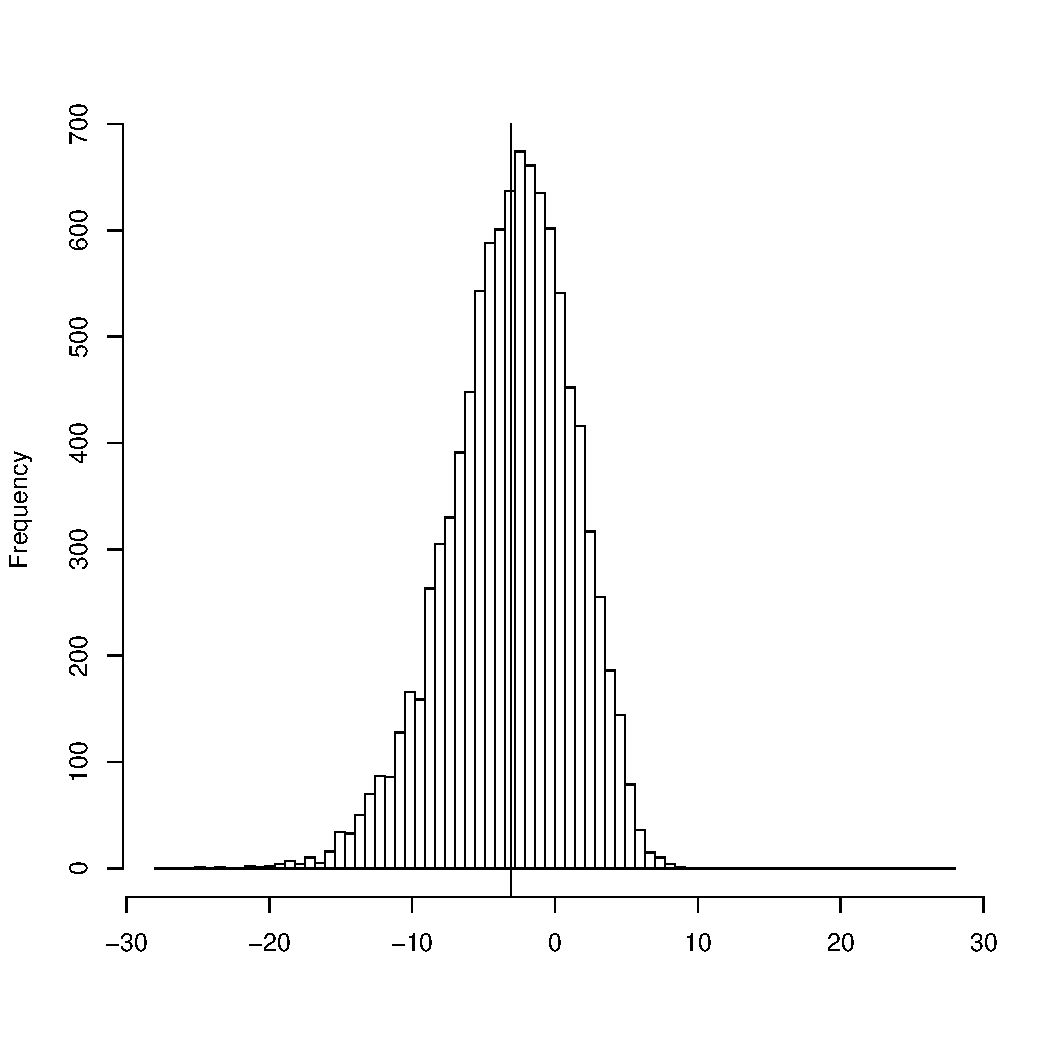
\includegraphics[scale=1.0]{../scripts/mtdna/uncentered1-2hist.pdf}}}
	  \put(250,-490){\normalsize$\delta(T_1,T_2 \mid X^{\ast})$}
\end{picture}

\myNewSlide
\section*{RELL bootstrap}
\large
Often, the MLE of numerical parameters (including branch lengths) do not change much when we bootstrap.

So, we can simply resample the site $\ln L$ values and sum them (rather than reoptimizing parameters).

This is called the RELL bootstrap \citep[][and Felsenstein]{KishinoMH1990}. It is not a ``safe'' replacement for normal bootstrapping \citep[especially on large trees;][]{StamatakisHR2008} when you want to estimate clade support.

But it should be good enough for helping us learn about the standard error of the $\ln L$.

And it is really fast.

\myNewSlide
\begin{picture}(500,0)(0,0)
	  \put(0,10){\large The (RELL) bootstrapped sample of statistics.}
	  \put(0,-20){\large Is this the null distribution for our $\delta$ test statistic?}
	  \put(20,-250){\makebox(0,0)[l]{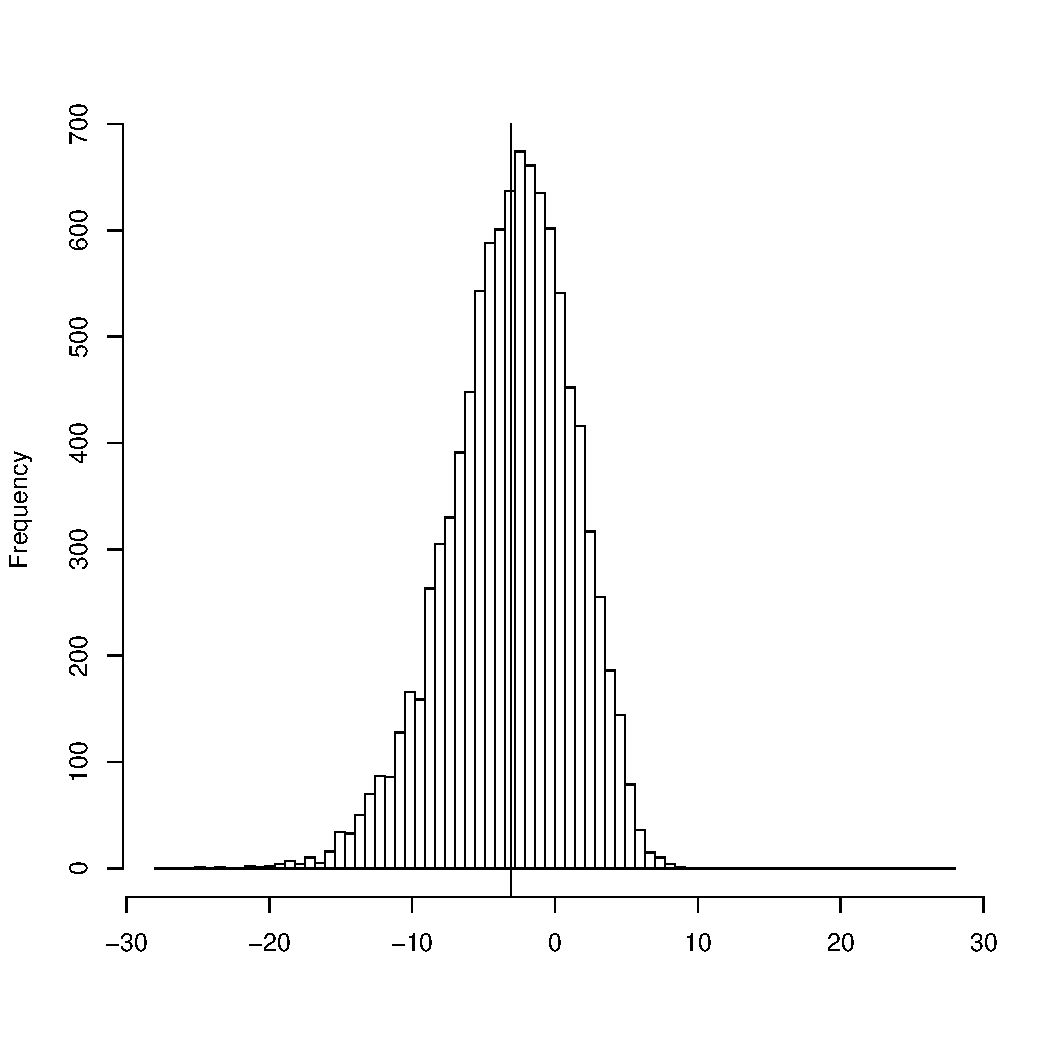
\includegraphics[scale=1.0]{../scripts/mtdna/uncentered1-2hist.pdf}}}
	  \put(250,-490){\normalsize$\delta(T_1,T_2 \mid X^{\ast})$}
\end{picture}

\myNewSlide
\section*{KH Test - `centering'}
$H_0$ gives us the expected value: $$\mathbb{E}_{H_0}\left[\delta(T_1,T_2 \mid X)\right] = 0$$
Bootstrapping gives us a reasonable guess of the variance under $H_0$

By subtracting the mean of the bootstrapped $\delta(T_1,T_2 \mid X^{\ast})$ values, we can create a null distribution.

For each of the $j$ bootstrap replicates, we treat $$\delta(T_1,T_2 \mid X^{\ast j}) - \bar\delta(T_1,T_2 \mid X^{\ast})$$  as draws from the null distribution.

\myNewSlide
\begin{picture}(500,0)(0,0)
	  \put(0,10){\large $\delta(T_1,T_2 \mid X^{(j)})-\bar\delta(T_1,T_2 \mid X^{\ast})$}
	  \put(0,-25){for many (RELL) bootstrapped replicates of the data}
	  \put(20,-250){\makebox(0,0)[l]{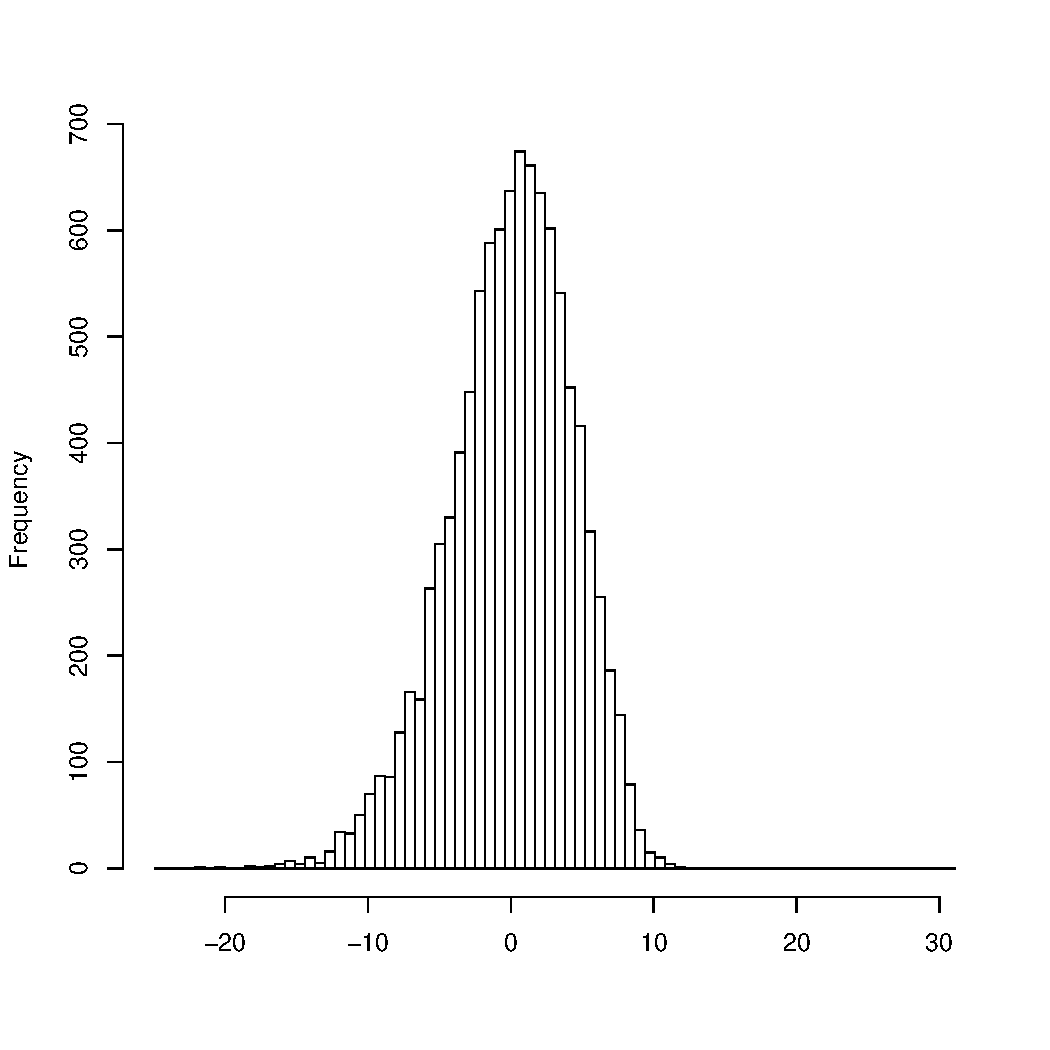
\includegraphics[scale=1.0]{../scripts/mtdna/centered1-2hist.pdf}}}
	  \put(150,-490){\normalsize$\delta(T_1,T_2 \mid X^{(j)})-\bar\delta(T_1,T_2 \mid X^{\ast})$}
\end{picture}

\myNewSlide
\begin{picture}(500,0)(0,0)
	  \put(0,10){Approximate null distribution with}
	  \put(0,-30){tails (absolute value $\geq 3.18$) shown}
	  \put(20,-250){\makebox(0,0)[l]{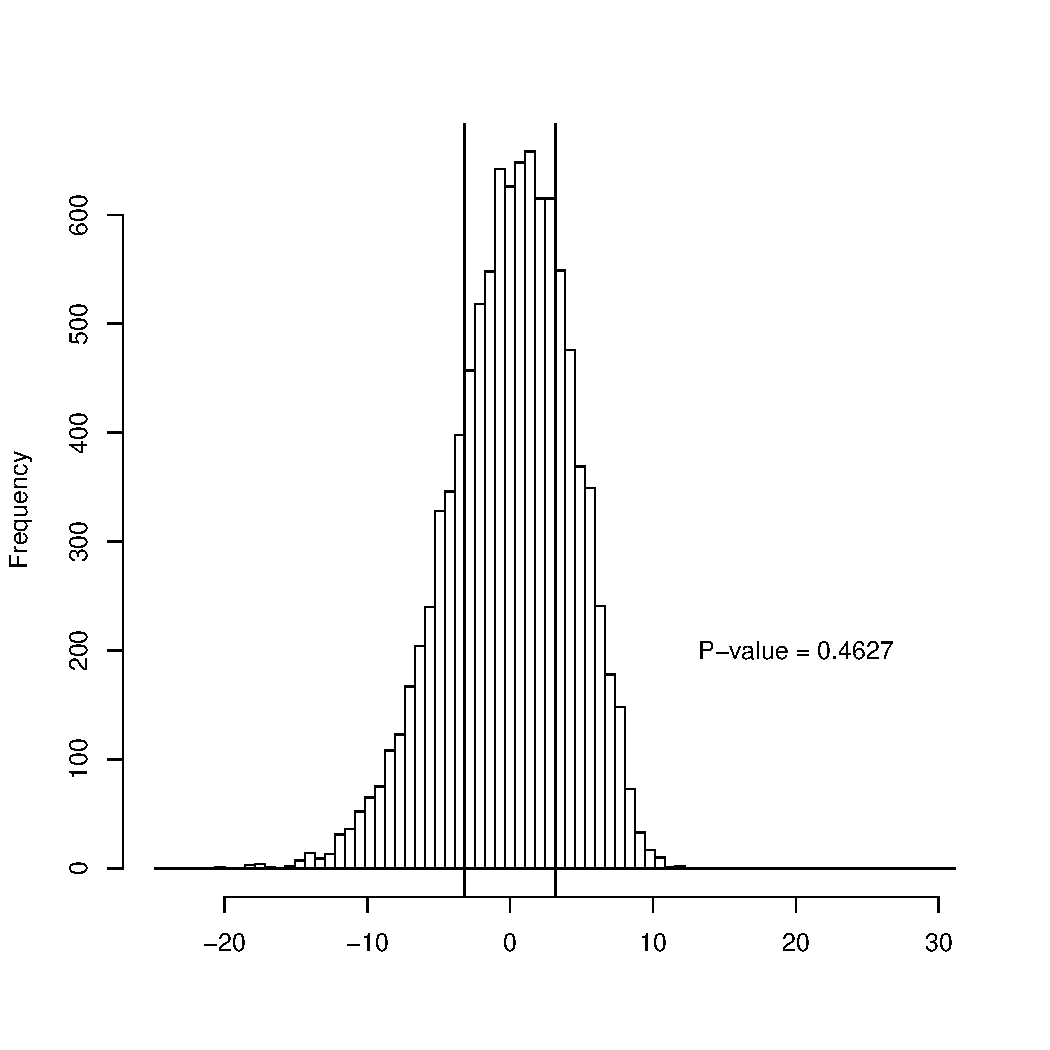
\includegraphics[scale=1.0]{../scripts/mtdna/centered1-2hist-p.pdf}}}
	  \put(175,-490){\normalsize$\delta(T_1,T_2 \mid X^{\ast})-\bar\delta(T_1,T_2 \mid X^{\ast})$}
\end{picture}


\myNewSlide
\section*{Summary - Part 1}

\begin{itemize}
	\item $\delta(T_1,T_2 \mid X) = 2\left[\ln L(T_1 \mid X) - \ln L(T_2 \mid X)\right]$ is a powerful statistic for discrimination between trees.
	\item We can assess confidence by considering the variance in signal between different characters.
	\item Bootstrapping helps us assess the variance in $\ln L$ that we would expect to result from sampling error.
\end{itemize}

\myNewSlide
\section*{Scenario}
\begin{enumerate}
	\item A (presumably evil) competing lab scoops you by publishing a tree, $T_1$, for your favorite group of organisms.
	\item You have just collected a new dataset for the group, and your ML estimate of the best tree, $T_2$, differ's from $T_1$.
	\item A KH Test shows that your data {\bf significantly} prefer $T_2$ over $T_1$.
	\item You write a (presumably scathing) response article.
\end{enumerate}
Should a {\em Systematic Biology} publish your response?

\myNewSlide
\section*{What if start out with only one hypothesized tree, and we want to compare it to the ML tree?}
The KH Test is {\bf NOT} appropriate in this context \citep[see][for discussion of this point]{GoldmanAR2000}
	
{\bf Multiple Comparisons}: lots of trees increases the variance of $\delta(\hat{T},T_1 \mid X)$\\

{\bf Selection bias}: Picking the ML tree to serve as one of the hypotheses invalidates the centering procedure of the KH test.

\myNewSlide
\section*{Using the ML tree in your test introduces selection bias}
Even when the $H_0$ is true, we do not expect $2\left[\ln L(\hat{T}) - \ln L(T_1)\right]= 0$

Imagine a competition in which a large number of equally skilled people compete, and you compare the score of one competitor against the highest scorer.

\myNewSlide
\begin{picture}(500,0)(0,0)
	  \put(-10,15){Experiment: 70 people each flip a fair coin 100 times and}
	  \put(0,-20){count \# heads.}
	  \put(100,-55){$h_1 - h_2$}
	  %\put(400,-55){$\max(h) - h_1$}
	  \put(-30,-250){\makebox(0,0)[l]{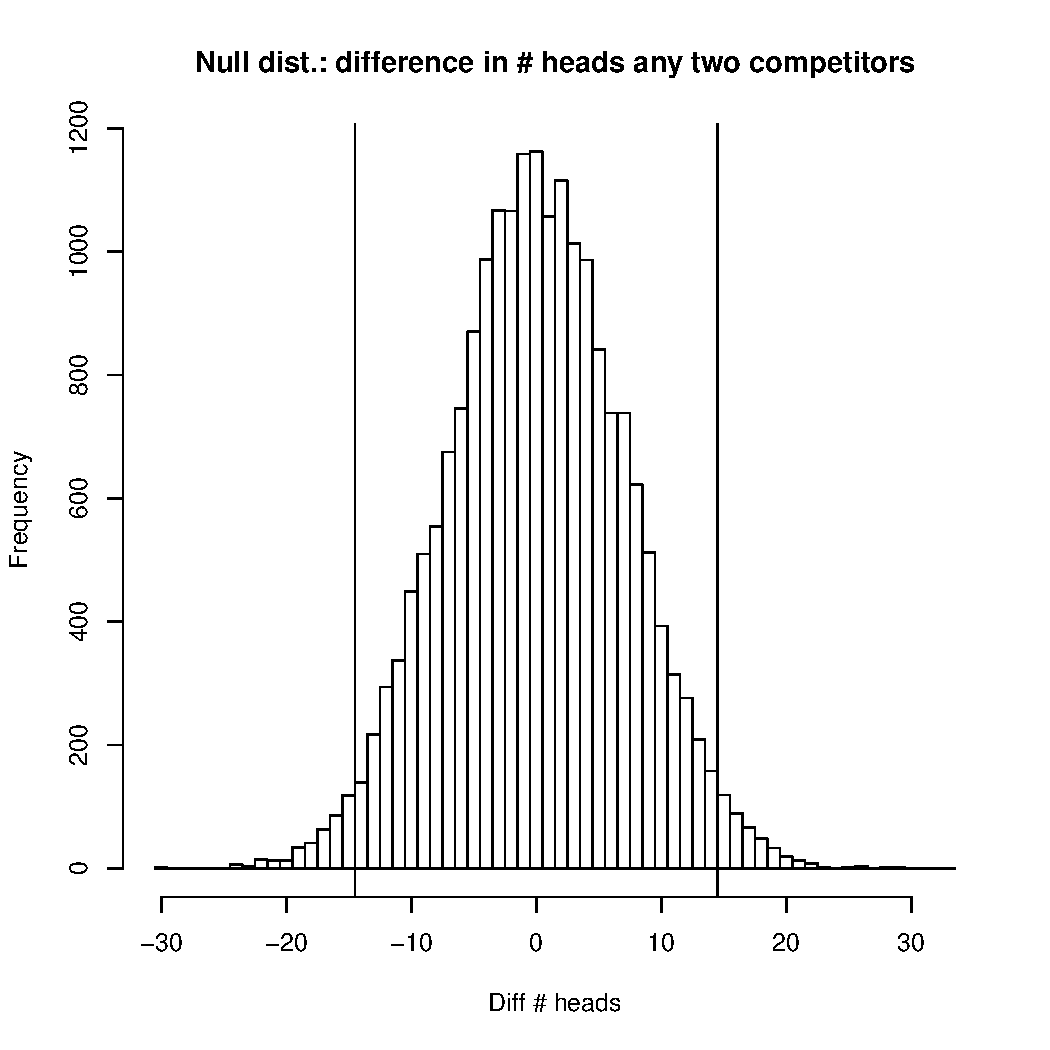
\includegraphics[scale=.75]{../scripts/cfc_diff_a_priori.pdf}}}
\end{picture}

\myNewSlide
\begin{picture}(500,0)(0,0)
	  \put(-10,15){Experiment: 70 people each flip a fair coin 100 times and}
	  \put(0,-20){count \# heads.}
	  \put(100,-55){$h_1 - h_2$}
	  \put(400,-55){$\max(h) - h_1$}
	  \put(-30,-250){\makebox(0,0)[l]{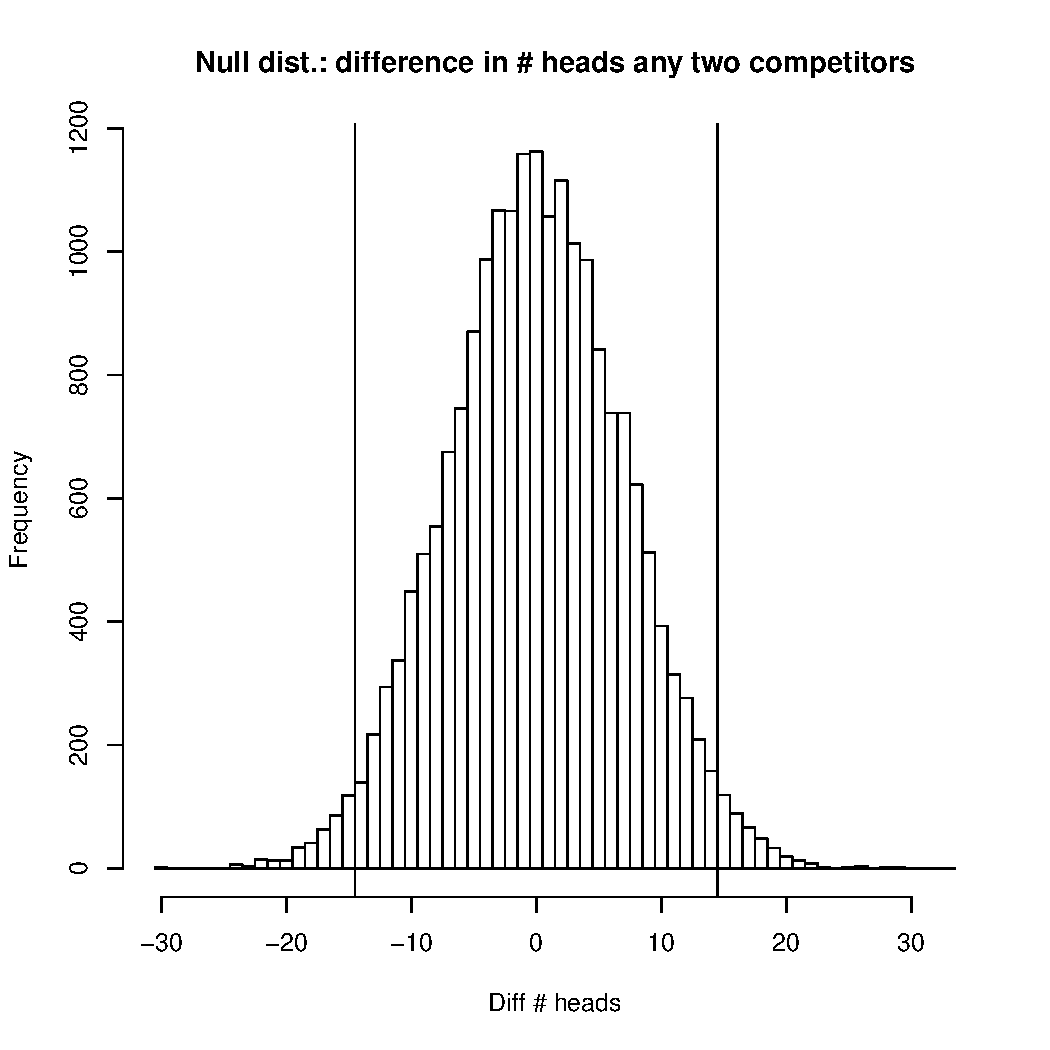
\includegraphics[scale=.75]{../scripts/cfc_diff_a_priori.pdf}}}
	  \put(320,-250){\makebox(0,0)[l]{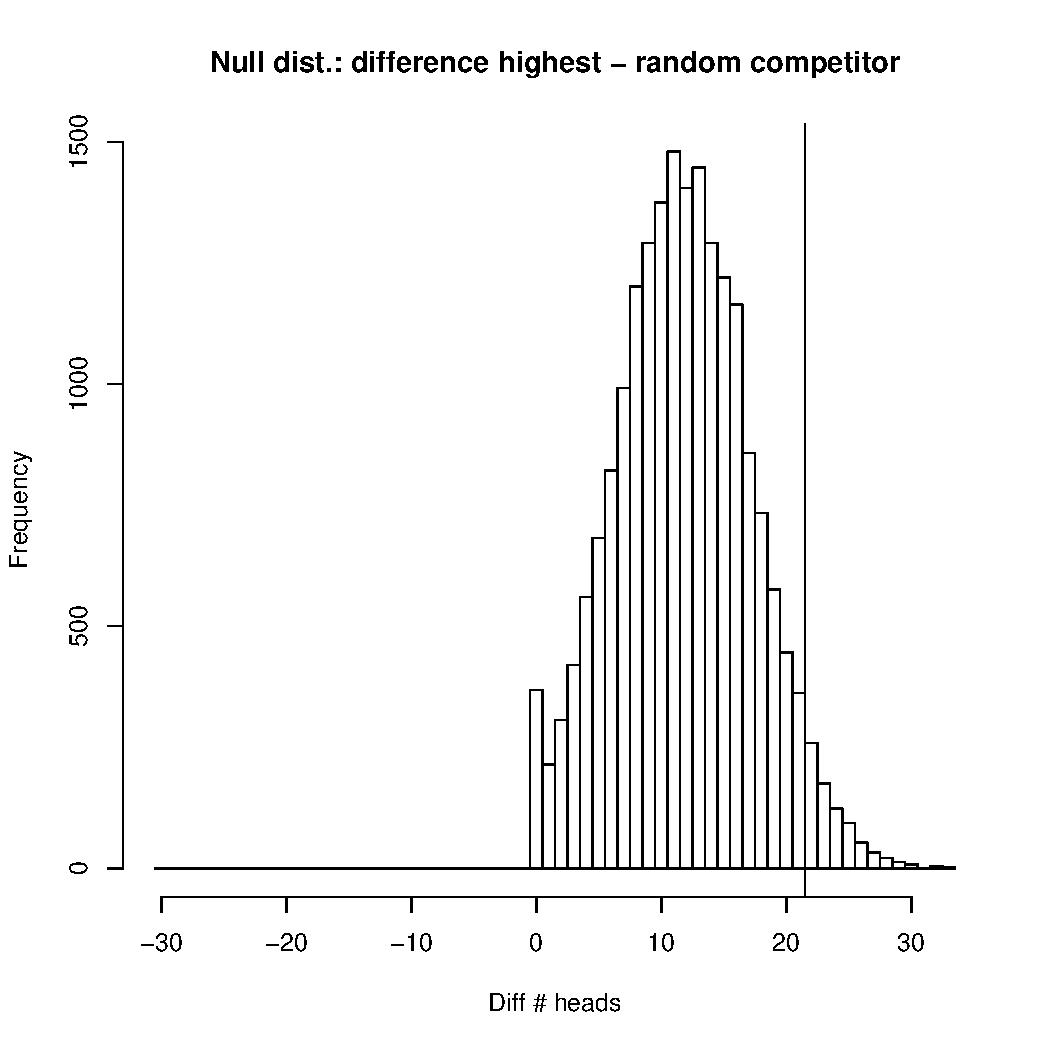
\includegraphics[scale=.75]{../scripts/cfc_diff_best_v_one.pdf}}}
\end{picture}


\myNewSlide 
\section*{Shimodaira and Hasegawa proposed the SH test which deals the ``selection bias'' introduced by using the ML tree in your test}
You have to specify of a {\bf set of candidate trees} - inclusion in this set {\bf must not} depend on the dataset to be analyzed.

The null hypothesis is that all members of the candidate set have the same expected score.

The test makes worst-case assumptions, so the SH test {\bf is conservative}.

\myNewSlide
\section*{SH test candidate set selection}
\large
\begin{itemize}
	\item Should be all trees that you would have seriously entertained before seeing the data (considering a subset of trees for computational convenience can invalidate the test).
	\item Using all trees is safe.
	\item If a tree has low $\ln L$ and low variance of site-log-likelihoods then it can probably be safely removed without affecting the $P$-values of other trees\footnote{Because such a tree would be unlikely to ever be the tree that is the determines the maximum diplacement from the centered value, $m^{(j)}$.}
\end{itemize}

\myNewSlide
{\bf SH Test details}
\normalsize
\begin{compactitem}
	\item For each tree $T_i$ in the candidate set calculate $\delta(\hat{T}, T_i \mid X)$
	\item Bootstrap to generate ${\ln L}(T_i \mid X^{(j)})$ for each bootstrap replicate $j$.
	\item For each tree $T_i$, use the mean, $\bar{\ln L}(T_i \mid X^{\ast})$, over all bootstrap replicates to center the bootstrapped collection of log-likelihoods:
		$$c_i^{(j)} = {\ln L}(T_i \mid X^{(j)})-\bar{\ln L}(T_i \mid X^{\ast})$$
	\item For each bootstrap replicate, $j$, pick the highest value from the centered distributions (this mimics the selection bias): $$m^{(j)} = \max\left[c_i^{(j)}\right] \mbox{ over all } i$$
	\item Then for each tree and replicate, you get a sample from the null $\delta_i^{(j)} = m^{(j)} - c_i^{(j)}$
	\item $P$-value for tree $T_i$ is approximated by the proportions of bootstrap reps for which: $$\delta_i^{(j)} \leq \delta(\hat{T}, T_i \mid X)$$
\end{compactitem}


\myNewSlide
\large
\begin{picture}(500,0)(0,0)
	  \put(-200,-190){\makebox(0,0)[l]{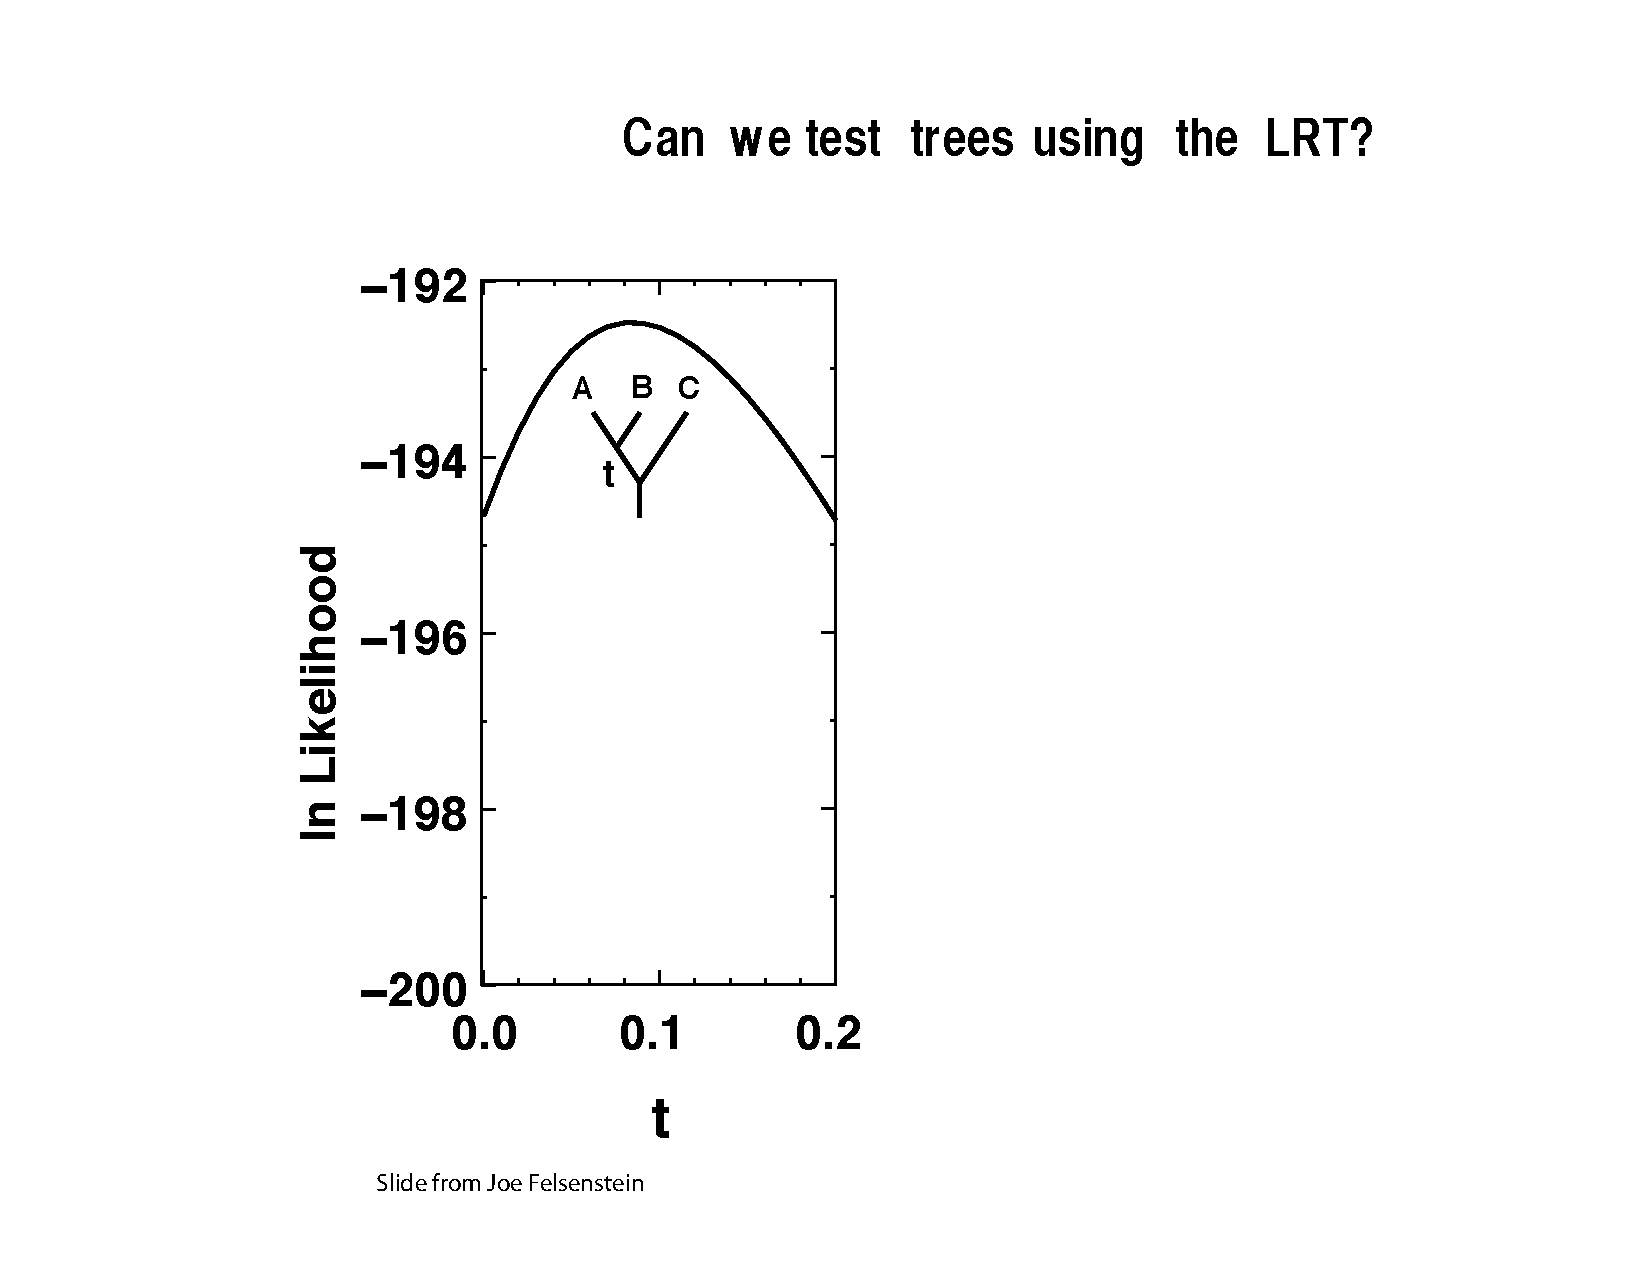
\includegraphics[scale=1.0]{../newimages/JoeFelsTreeLRT1.pdf}}}
	  \put(250,-100){1. Should we calculate the LRT as:}
	  \put(224,-140){$\delta_i = 2\left[\ln L(t=\hat{t},T_i \mid X) - \ln L(t=0,T_i \mid X)\right]$}
	  \put(250,-250){2. And can we use the $\chi_1^2$ distribution to}
	  \put(250,-290){get the critical value for $\delta$?}
\end{picture}

\myNewSlide
\begin{picture}(500,0)(0,0)
	  \put(-200,-190){\makebox(0,0)[l]{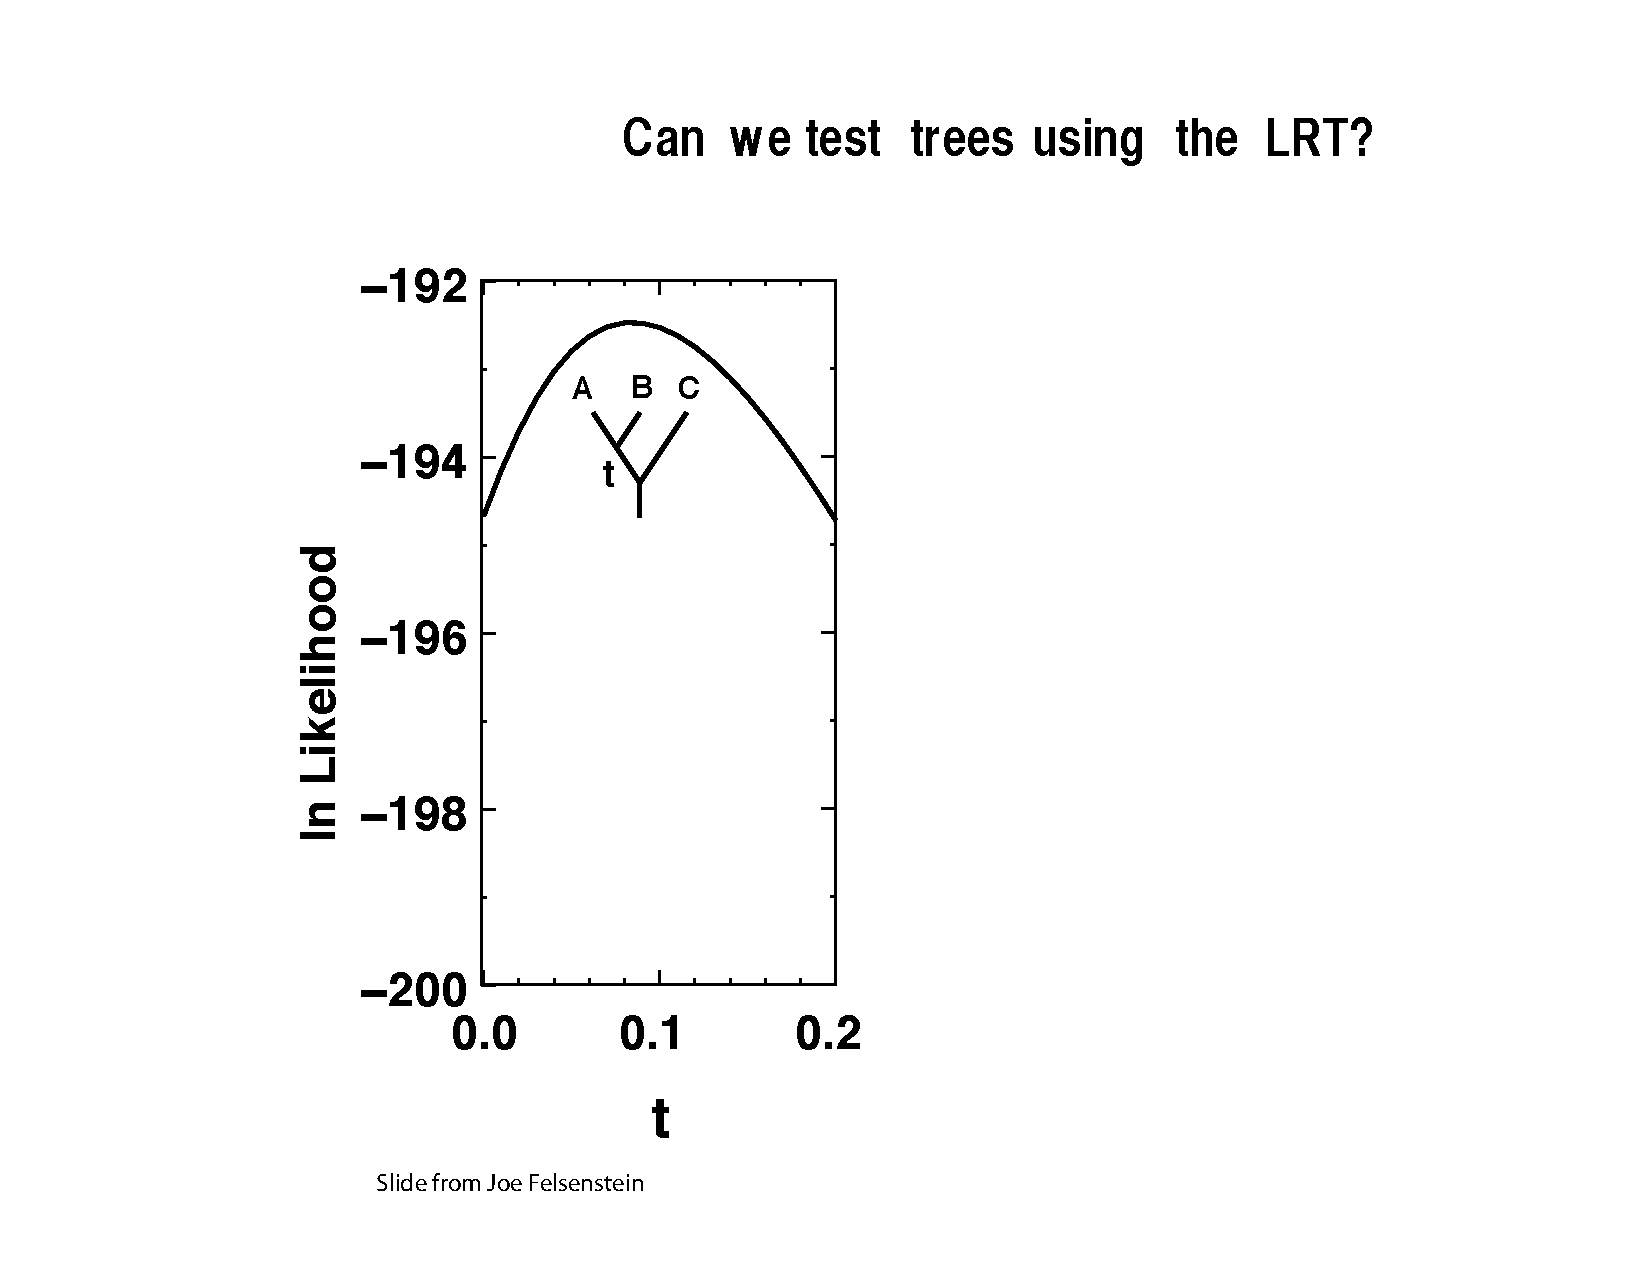
\includegraphics[scale=1.0]{../newimages/JoeFelsTreeLRT1.pdf}}}
	  \put(250,-100){1. Should we calculate the LRT as:}
	  \put(224,-140){$\delta_i = 2\left[\ln L(t=\hat{t},T_i \mid X) - \ln L(t=0,T_i \mid X)\right]$}
	  \put(250,-180){{\bf \color{red}No. $t=0$ might not yield the best}}
	  \put(260,-220){\bf\color{red} alternative $\ln L$}
	  \put(250,-290){2. And can we use the $\chi_1^2$ distribution to}
	  \put(250,-330){get the critical value for $\delta$ ?}
	  \put(250,-370){{\bf \color{red}No. Constraining parameters}}
	  \put(260,-410){{\bf \color{red}at boundaries leads to a mixture}}
	  \put(260,-450){{\bf \color{red}such as: $\frac{1}{2}\chi_0^2 + \frac{1}{2}\chi_1^2$}}
	  \put(260,-490){\small See \citet{OtaWHSK2000}.}
\end{picture}

\myNewSlide
\begin{picture}(500,0)(0,0)
	  \put(-200,-190){\makebox(0,0)[l]{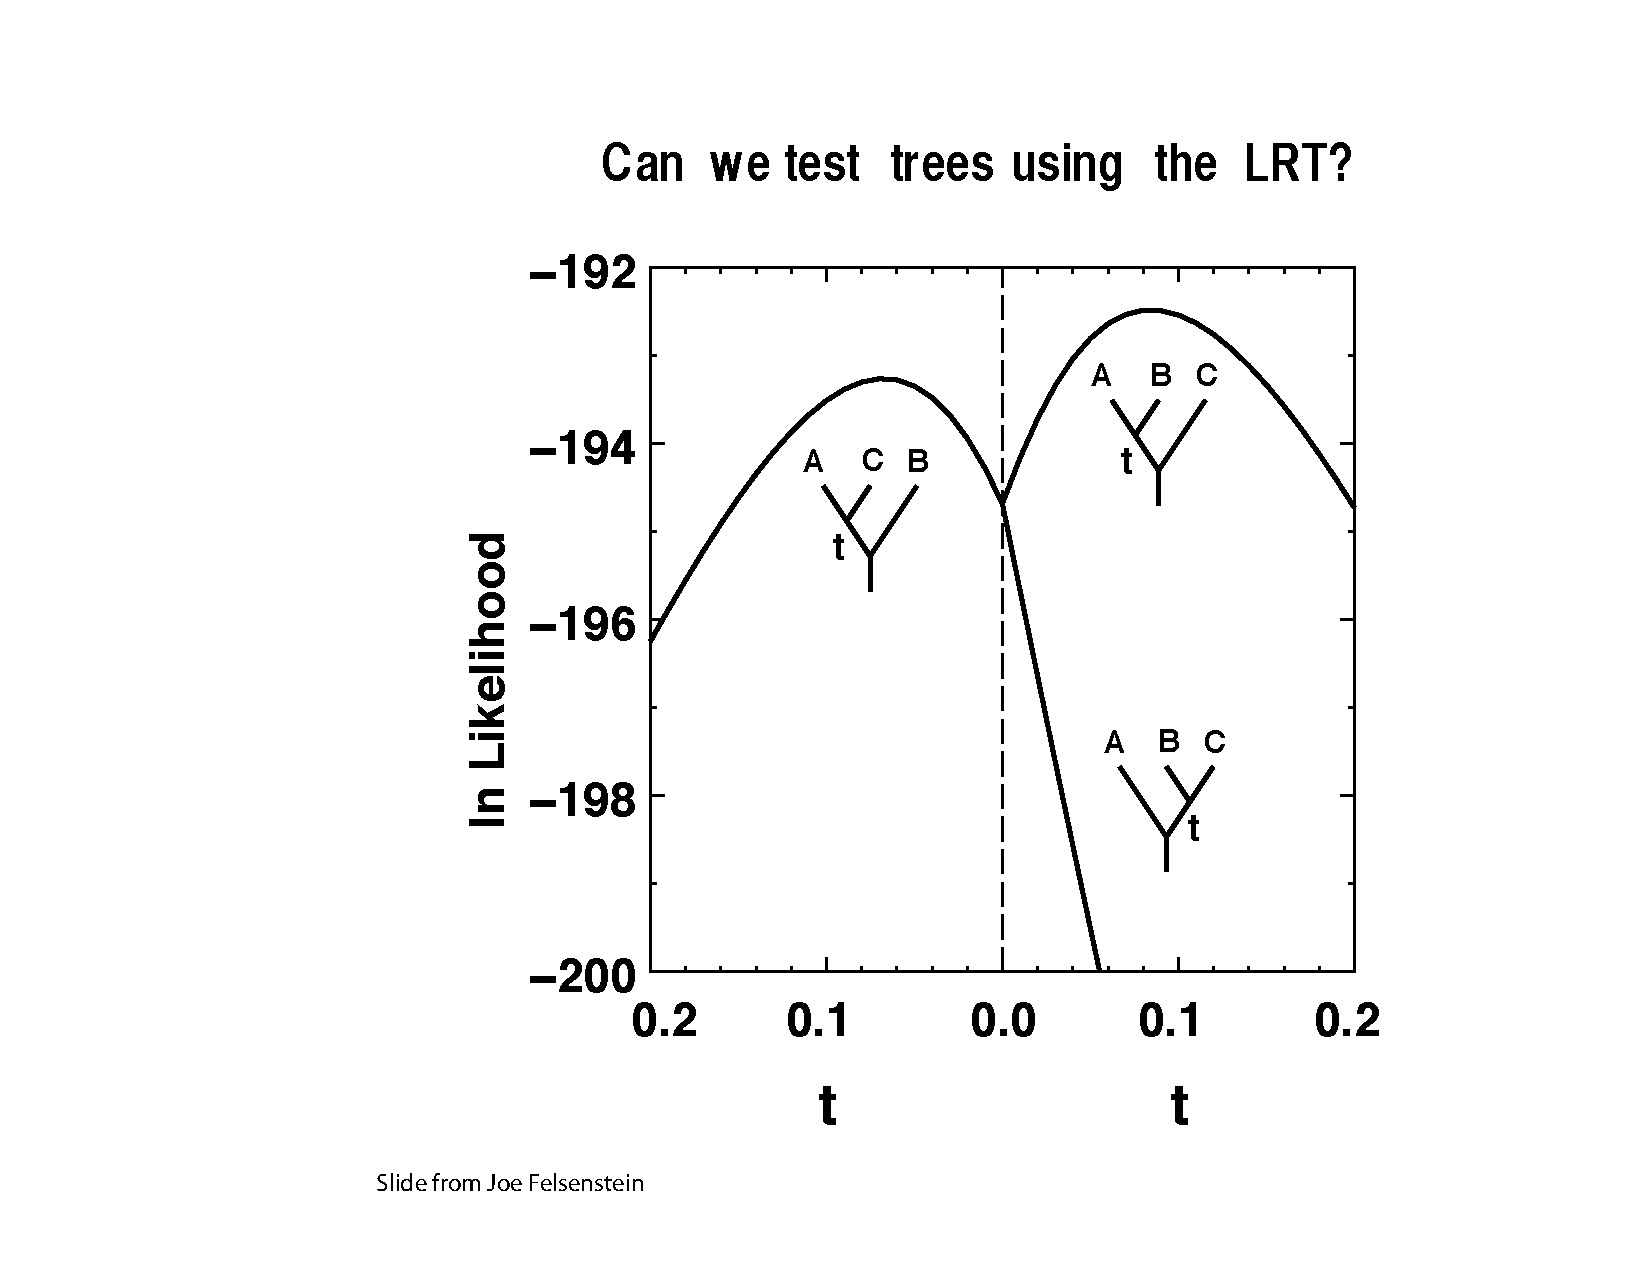
\includegraphics[scale=1.0]{../newimages/JoeFelsTreeLRT2.pdf}}}
	  \put(470,-170){{\bf \color{red}No, tree hypotheses}}
	  \put(470,-200){{\bf \color{red}are not nested! }}
\end{picture}

\myNewSlide
\section*{Another ways to assess the null distribution of the LR test statistic}
\begin{itemize}
	\item Bootstrapping then centering LR, and 
	\item Using normality assumptions.
\end{itemize}
are both clever and cute solutions.

But they do not match the null distribution under any model of sequence evolution.

\myNewSlide
\section*{Parametric bootstrapping to generate the null distribution for the LR statistic}
\begin{enumerate}
	\item find the best tree and model pair that are consistent with the null,
	\item Simulate many datasets under the parameters of that model,
	\item Calculate $\delta^{(j)} = 2\left[\ln L (\hat{T}^{(j)} \mid  X^{(j)}) - \ln L (\hat{T}_{0}^{(j)} \mid  X^{(j)})\right]$ for each simulated dataset.
		\begin{compactitem}
			\item the $(j)$ is just an index for the simulated dataset,
			\item $\hat{T}_{0}^{(j)}$ is the tree under the null hypothesis for simulation replicate $j$
		\end{compactitem}
\end{enumerate}

\myNewSlide
\section*{Parametric bootstrapping}
This procedure is often referred to as SOWH test (in that form, the null tree is specified {\em a priori}).

\citet{HuelsenbeckHN1996} describes how to use the approach as a test for monophyly.

Intuitive and powerful, but not robust to model violation \citep{Buckley2002}.

Detailed step-by-step instructions in \url{https://molevol.mbl.edu/wiki/index.php/ParametricBootstrappingLab}

\myNewSlide
\includepdf[pages={1}]{/home/mholder/Documents/ku_teaching/BIOL-848-2013/images/gtr_i_g_sim_hist_data.pdf} 


\myNewSlide
\includepdf[pages={1}]{/home/mholder/Documents/ku_teaching/BIOL-848-2013/images/jc_sim_hist_data.pdf} 

\myNewSlide
\section*{aLRT of \citet{AnisimovaG2006}}
\begin{compactitem}
	\item For a {\bf branch} $j$, calculate $\delta_{j}^{\dag}$ as twice the difference in $\ln L$ between the optimal tree (which has the branch) and the best NNI neighbor.
	\item This is very fast.
	\item They argue that the null distribution for each LRT around the polytomy follows a $\frac{1}{2}\chi_0^2 + \frac{1}{2}\chi_1^2$ distribution
	\item The introduce Bonferroni-correction appropriate for correcting for the selection of the best of the three resolutions.
	\item They find aLRT to be accurate and powerful in simulations, but \citet{AnisimovaGDDG2011} report that it rejects too often and is sensitive to model violation.
\end{compactitem}

\myNewSlide
\begin{picture}(500,0)(0,0)
	  \put(-130,-450){\makebox(0,0)[l]{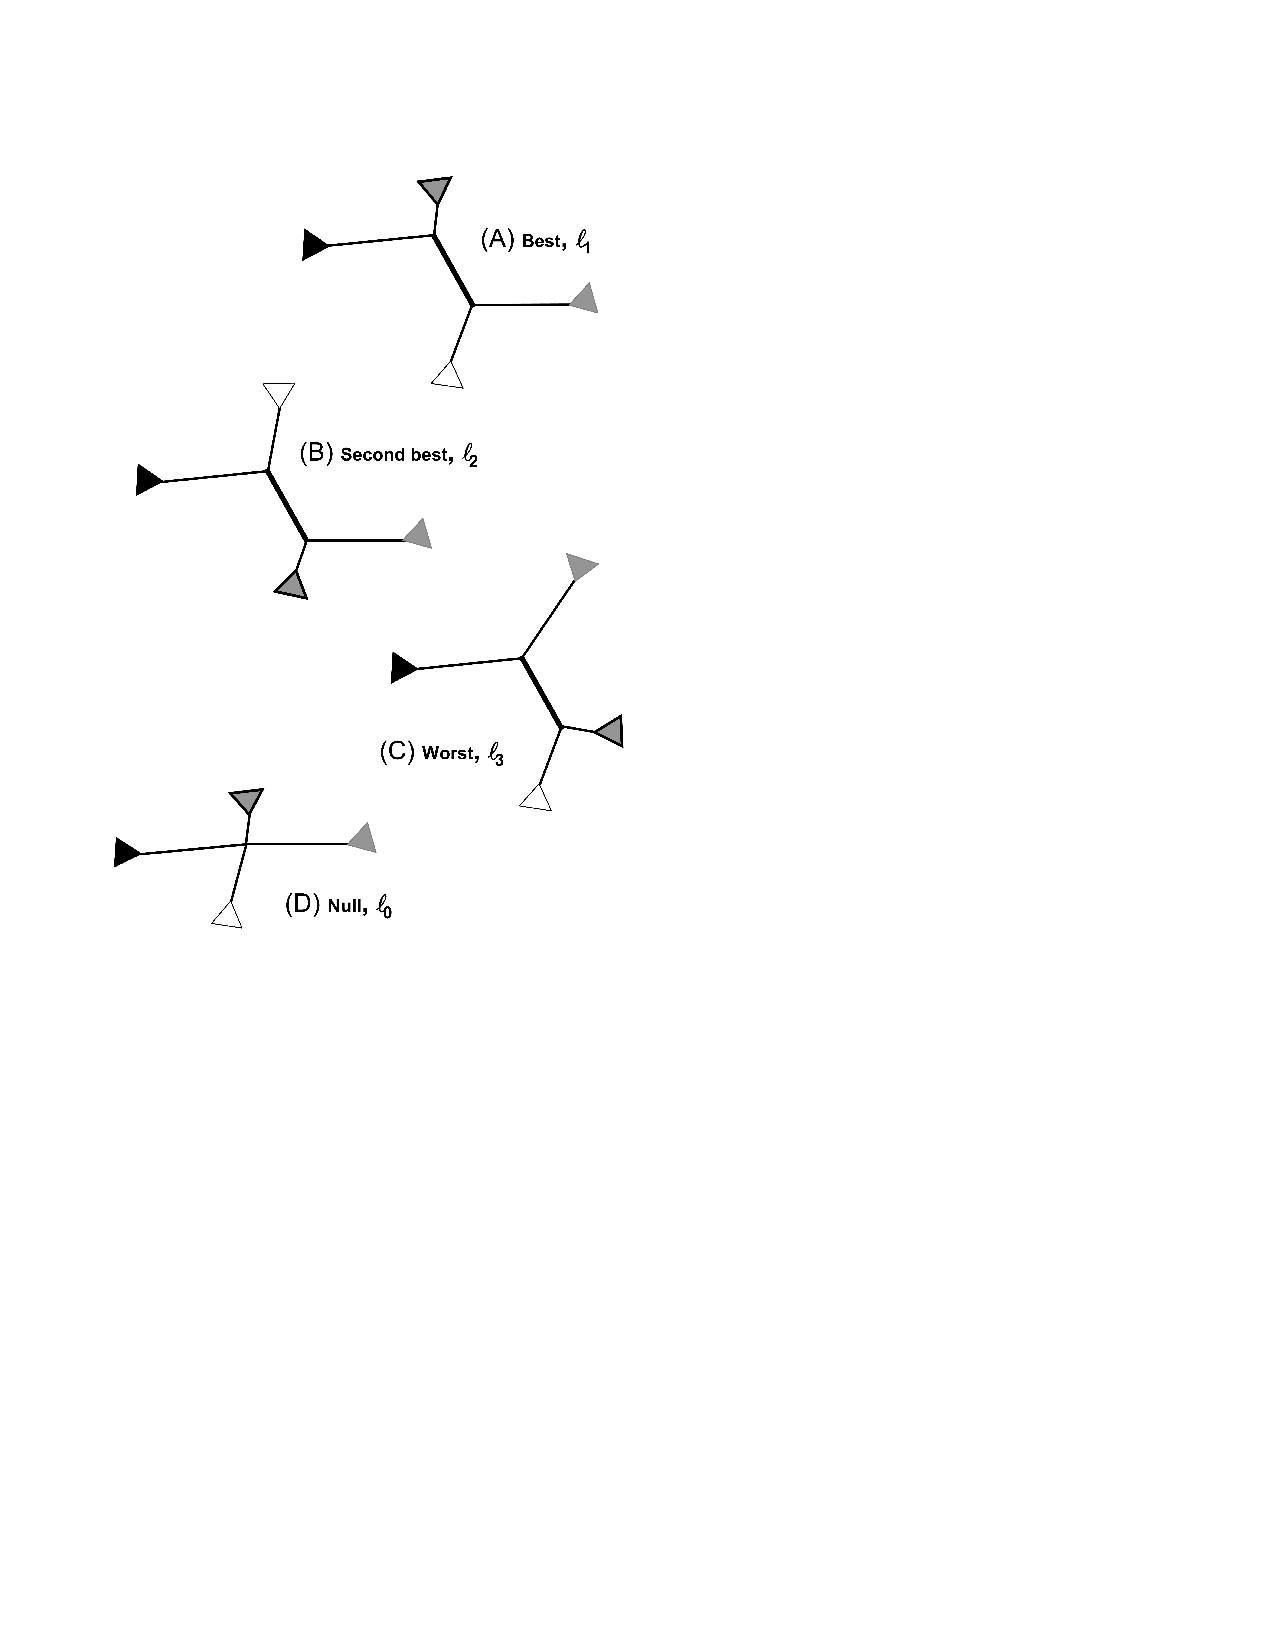
\includegraphics[scale=1.5]{../newimages/AnisimovaG2006Fig1.pdf}}}
	  \put(300,-200){aLRT = $2\left[\ln \ell_1 - \ln L(T_2 \mid X)\right]$}
	  \put(300,-240){$\ell_1 = L(T_1 \mid X)$}
	  \put(400,-400){\small Image from \citet{AnisimovaG2006}}
\end{picture}

\myNewSlide
\section*{aBayes \citet{AnisimovaGDDG2011} }


$$\mbox{aBayes}(T_1 \mid X) = \frac{\Pr(X \mid T_1)}{\Pr(X \mid T_1) + \Pr(X \mid T_2) + \Pr(X \mid T_3)}$$

Simulation studies of \citet{AnisimovaGDDG2011} show it to have the best power of the methods that do not have inflated probability of falsely rejecting the null.

It is sensitive to model violation.

This is similar to ``likelihood-mapping'' of \citet{StrimmerVH1997}




\myNewSlide
\Large
Bootstrap proportions have been characterized as providing:
\begin{compactitem}
	\item a measure of repeatability,
	\item an estimate of the probability that the tree is correct (and bootstrapping has been criticized as being too conservative in this context),
	\item the P-value for a tree or clade
\end{compactitem}




\myNewSlide
\section*{coin flipping (yet again)}
$N=100$ and $H=60$

Can we reject the hypothesis of a fair coin?

We can use simulation to generate the null distribution (we could actually use the binomial distribution to analytically solve this one)...

\myNewSlide

\begin{picture}(0,0)(0,0)
	\put(-10,-250){\makebox(0,0)[l]{\includegraphics[scale=1.0]{/home/mholder/Documents/ku_teaching/BIOL-848-2013/images/nullhist.pdf}}}
	\put(150,-250){\color{red} P-value $\approx$ 0.029 }
\end{picture}

\myNewSlide
We discussed how bootstrapping gives us a sense of the variability ofour estimate

It can also give a tail probability for $\Pr(f_H^{(boot)} \leq 0.5)$

Amazingly (for many applications):
$$ \Pr(\hat{f}_H \geq 0.6 \mid \mbox{null is true}) \approx \Pr(f_H^{(boot)} \leq 0.5)$$

In other words, the $P$-value is approximate by the fraction of bootstrap replicates consistent with the null.
\myNewSlide

\begin{picture}(0,0)(0,0)
	\put(-60,-250){\makebox(0,0)[l]{\includegraphics[scale=1.0]{/home/mholder/Documents/ku_teaching/BIOL-848-2013/images/boothist.pdf}}}
	\put(30,-220){\color{red}$ \Pr(p^{(boot)} \leq 0.5)\approx$ 0.027 }
	\put(30,-265){\color{red}$ BP = \mbox{frac.~of } p^{(boot)} \geq 0.5$}
	\put(30,-310){\color{red}$ BP \approx 0.973$}
	\put(30,-345){\color{red}$ P\mbox{-value} \approx 1-BP$}
\end{picture}

\myNewSlide
\begin{picture}(-0,0)(-0,0)
	\put(60,00){\makebox(30,-150)[l]{\includegraphics[scale=0.5]{/home/mholder/Documents/ku_teaching/BIOL-848-2013/images/nullhist.pdf}}}
	\put(60,-260){\makebox(30,-150)[l]{\includegraphics[scale=0.5]{/home/mholder/Documents/ku_teaching/BIOL-848-2013/images/boothist.pdf}}}
\end{picture}







\myNewSlide
\begin{itemize}
	\item When you decide between trees, the boundaries between tree hypotheses can be curved 
	\item When the boundary of the hypothesis space is curved, 1 - BP can be a poor approximation of the $P$-value.
\end{itemize}
-- \citet{EfronHH1996}
\myNewSlide
\section*{\citet{EfronHH1996} view of tree space}
\begin{picture}(-0,0)(-0,0)
	\put(-10,-90){\makebox(30,-150)[l]{\includegraphics[scale=3]{/home/mholder/Documents/ku_teaching/BIOL-848-2013/images/EfronHH-treespace-fig.pdf}}}
\end{picture}

\myNewSlide
\section*{Parsimony-informative Pattern Frequency Space}
\begin{picture}(-0,0)(-0,0)
	\put(10,-140){\makebox(30,-150)[l]{\includegraphics[scale=1.]{/home/mholder/Documents/ku_teaching/BIOL-848-2013/images/simple-treespace.pdf}}}
\end{picture}
 
\myNewSlide
\begin{picture}(-0,0)(-0,0)
	\put(20,0){\normalsize Imagine hypothesis tests of locations with different border shapes:}
	\put(-10,-90){\makebox(30,-150)[l]{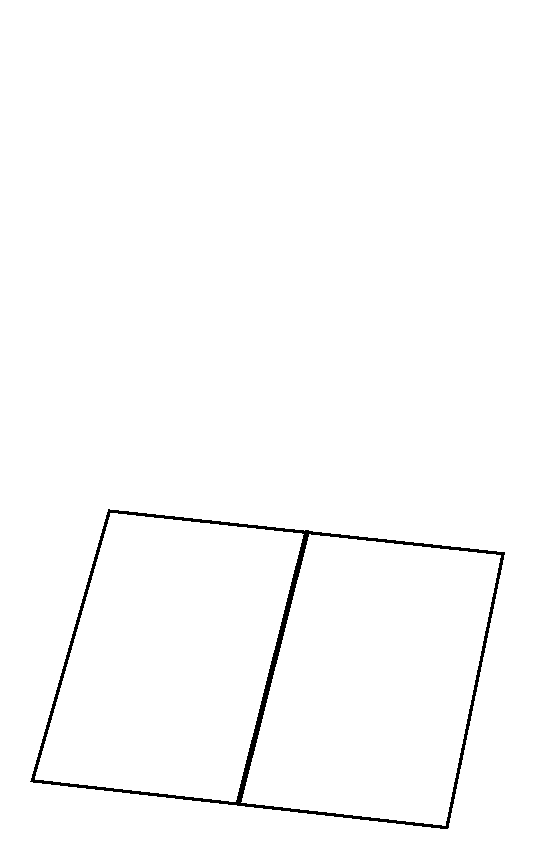
\includegraphics[scale=1.2]{../newimages/boundarylandscape.pdf}}}
	\put(300,-90){\makebox(30,-150)[l]{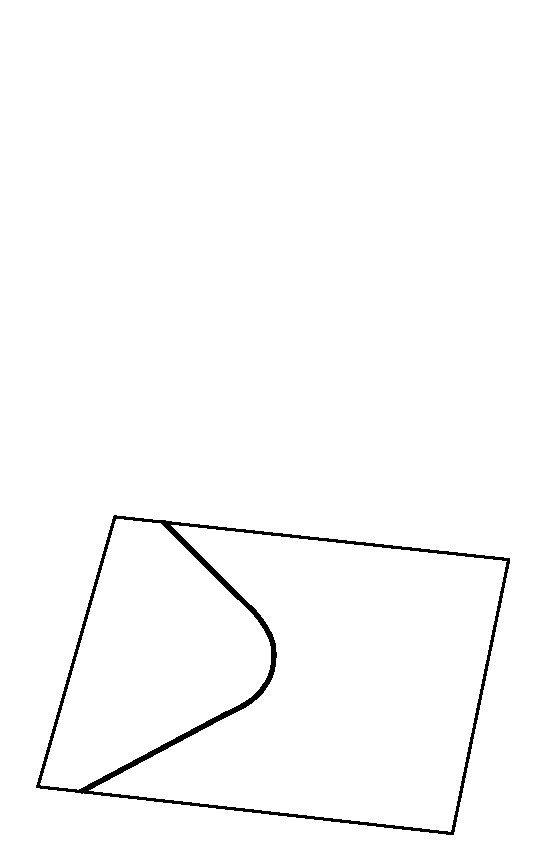
\includegraphics[scale=1.2]{../newimages/curved_boundarylandscape.pdf}}}
	\put(80,-290){$H_0$}
	\put(160,-330){$H_1$}
	\put(380,-290){$H_0$}
	\put(490,-330){$H_1$}
\end{picture}

\myNewSlide
\begin{picture}(-0,0)(-0,0)
	\put(40,0){\large Similar dataset with point estimates (red dot) in $H_1$}
	\put(20,-40){\large Green dot is the hardest set of locations in $H_0$ to reject.}
	\put(-10,-90){\makebox(30,-150)[l]{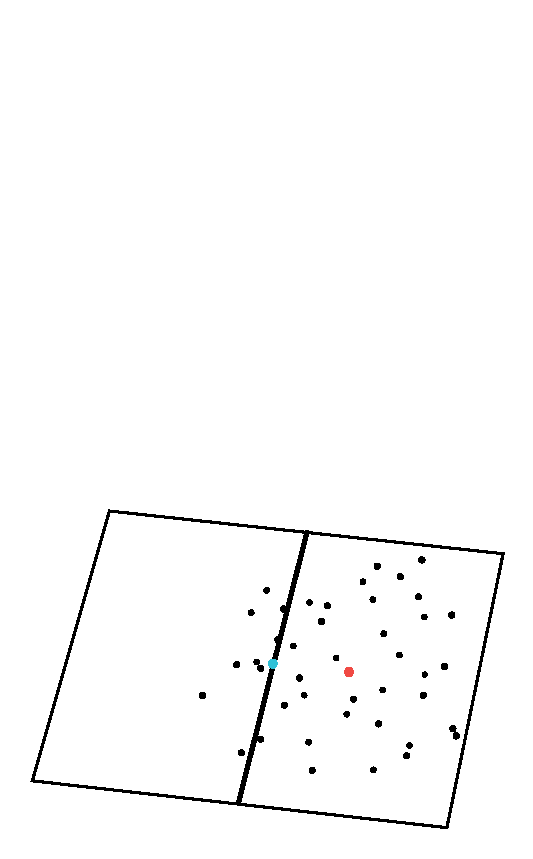
\includegraphics[scale=1.2]{../newimages/boundarylandscape_pts.pdf}}}
	\put(300,-90){\makebox(30,-150)[l]{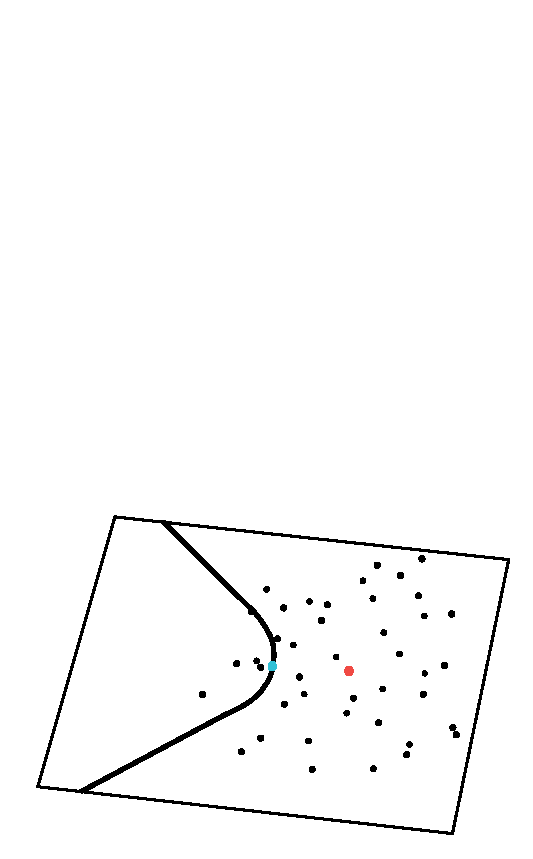
\includegraphics[scale=1.2]{../newimages/curved_boundarylandscape_pts.pdf}}}
\end{picture}

\myNewSlide
\begin{picture}(-0,0)(-0,0)
	\put(-10,-90){\makebox(30,-150)[l]{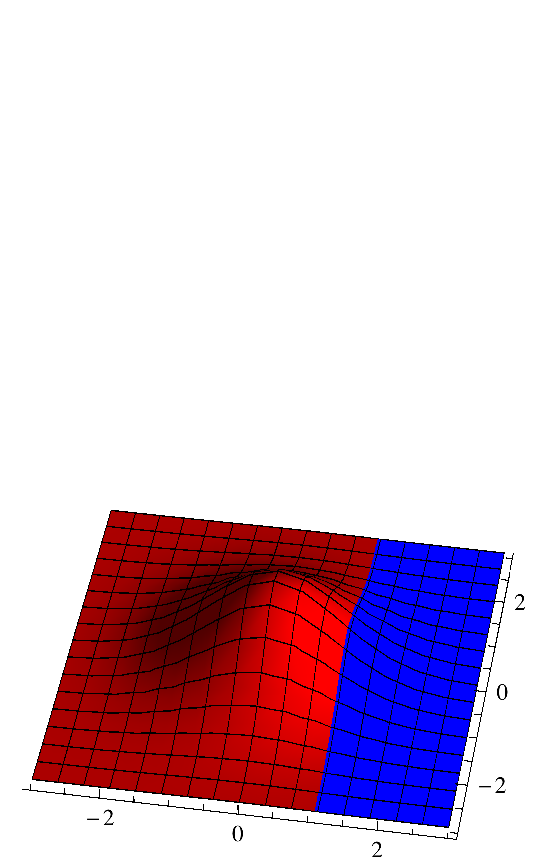
\includegraphics[scale=1.2]{../newimages/straight_p_value.pdf}}}
	\put(300,-90){\makebox(30,-150)[l]{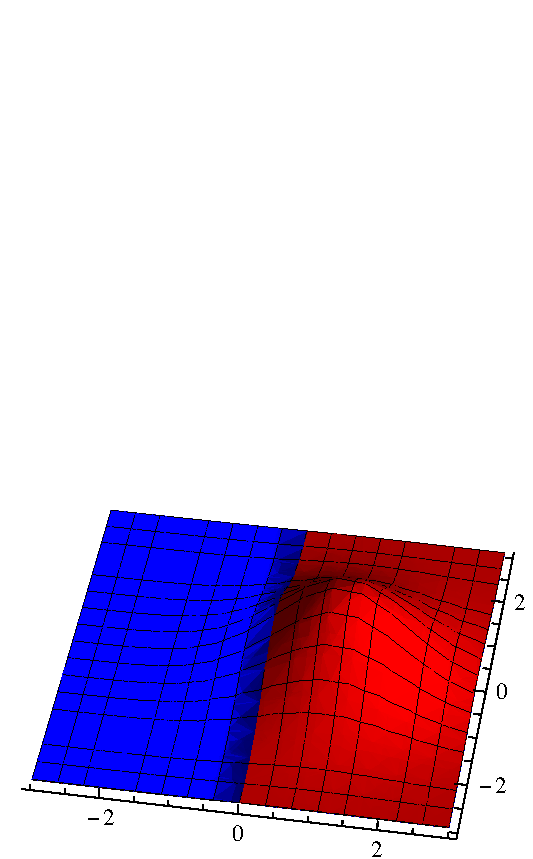
\includegraphics[scale=1.2]{../newimages/straight_boot_p_value.pdf}}}
	\put(40,0){\large In the straight border case, symmetry implies that:}
	\put(-20,-150){\large The actual $P$-value (blue region)}
	\put(420,-150){\large $\approx 1-BP$}
	\put(420,-190){\large ($1-BP$ is the blue below)}
\end{picture}
\myNewSlide
\begin{picture}(-0,0)(-0,0)
	\put(-10,-90){\makebox(30,-150)[l]{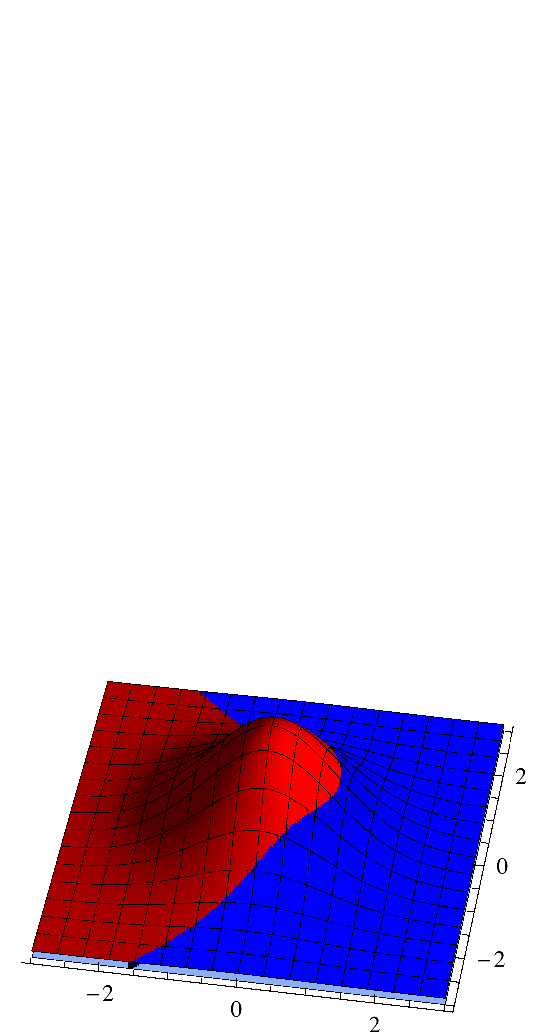
\includegraphics[scale=1.2]{../newimages/acurved_p_value.pdf}}}
	\put(300,-90){\makebox(30,-150)[l]{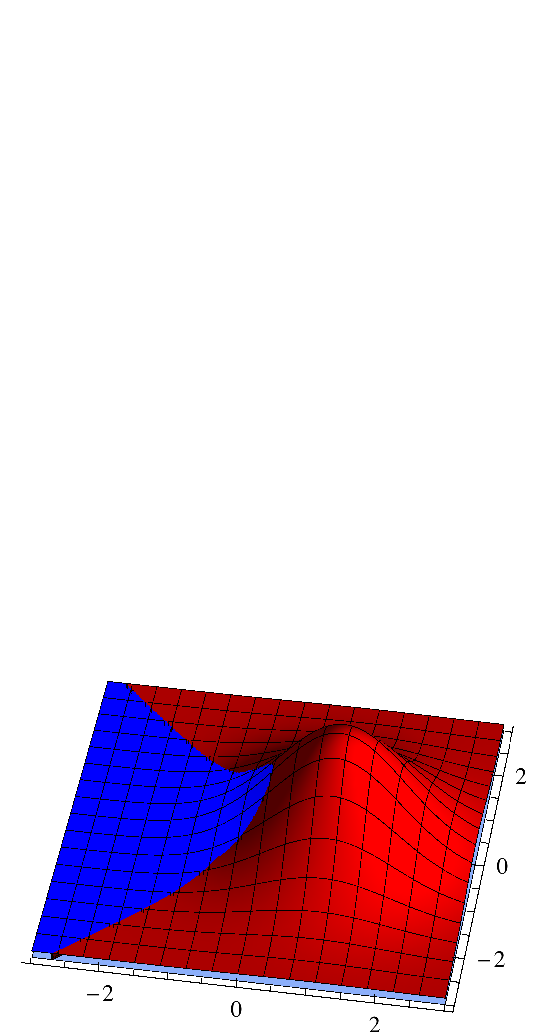
\includegraphics[scale=1.2]{../newimages/acurved_boot_p_value.pdf}}}
	\put(40,0){\large In the curved border case, the symmetry breaks down:}
	\put(-20,-150){\large The actual $P$-value (blue region)}
	\put(420,-150){\large $\neq 1-BP$}
	\put(420,-190){\large ($1-BP$ is the blue below)}
\end{picture}

\myNewSlide
\begin{itemize}
	\item \citet{EfronHH1996}  proposed a computationally expensive multi-level bootstrap (which has not been widely used).
	\item \citet{Shimodaira2002} used the same theoretical framework to devise a (more feasible) Approximately Unbiased (AU) test of topologies.
	\begin{itemize}
		\item Multiple scales of bootstrap resampling (80\% of characters, 90\%, 100\%, 110\%$\ldots$) are used to detect and correct for curvature of the boundary.
		\item Implemented in the new versions of PAUP$^{\ast}$
	\end{itemize}
\end{itemize}


\myNewSlide
\section*{\cite{Susko2010} adjusted BP -- aBP}
\large
\begin{compactitem}
	\item Susko agrees with curvature arguments of \citet{EfronHH1996} and \citet{Shimodaira2002}, {\bf but} points out that they ignore the {\bf sharp point} in parameter space around the polytomy.

	\item He correct bootstrap proportions:  $1-aBP$ accurately estimates the $P$-value.

	\item The method uses the multivariate normal distributions the based on calculations about the curvature of the {\em likelihood} surface.

	\item You need to perform a different correction when you know the candidate tree {\em a priori} versus when you are putting BP on the ML tree.

	\item BP may {\bf not} be conservative when you correct for selection bias.
\end{compactitem}

\myNewSlide
\begin{picture}(-0,0)(-0,0)
	\put(-60,-150){\makebox(30,-150)[l]{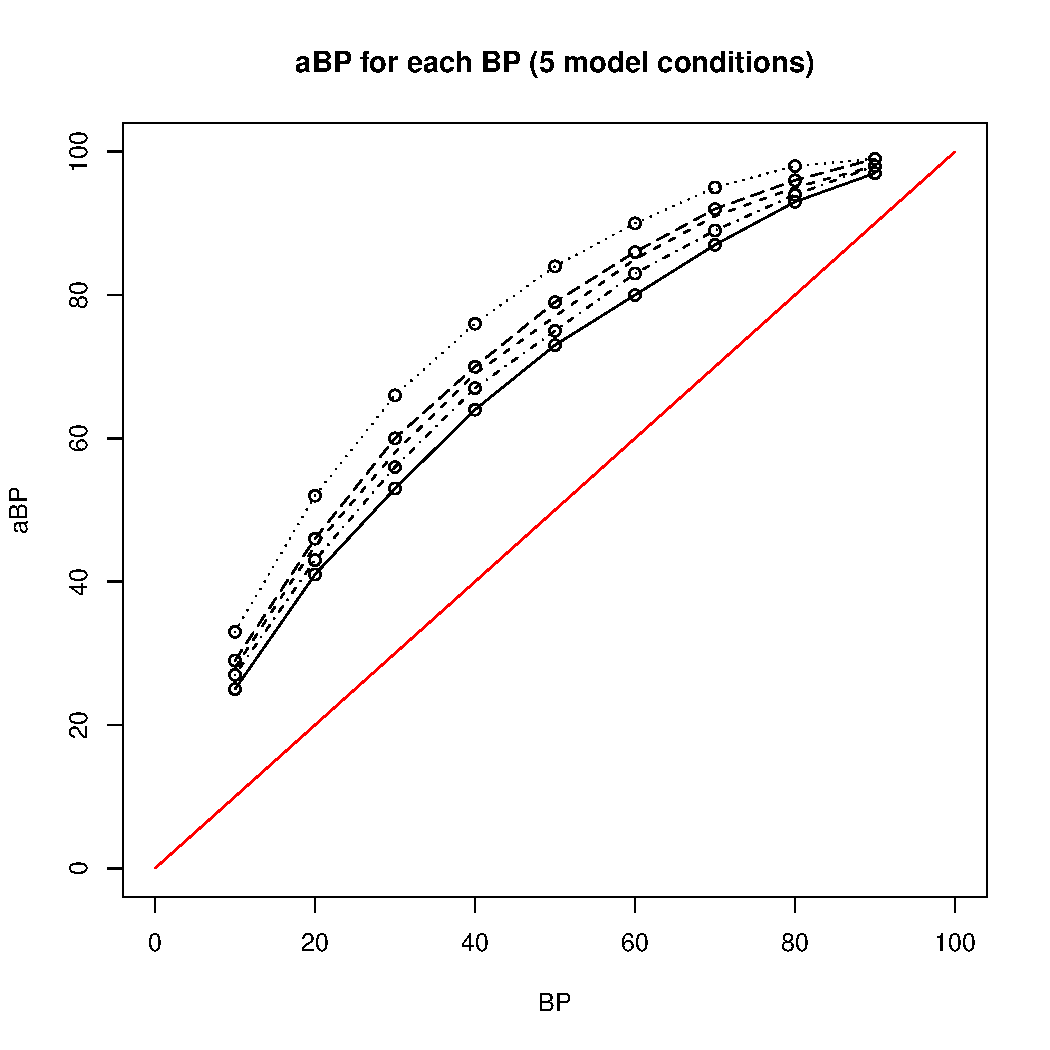
\includegraphics[scale=0.75]{../scripts/Susko2010Table3aBP.pdf}}}
	\put(300,-150){\makebox(30,-150)[l]{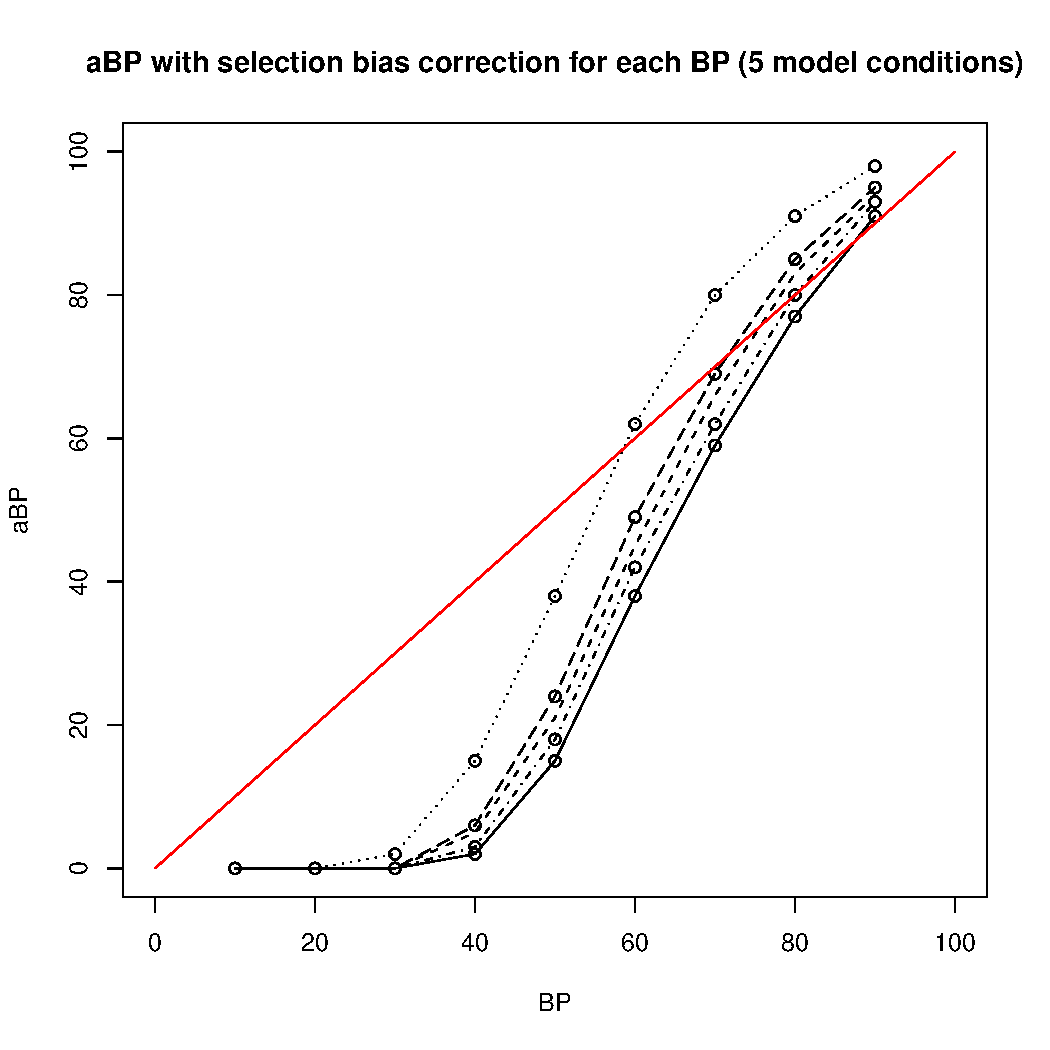
\includegraphics[scale=0.75]{../scripts/Susko2010Table3aBPMLCorrection.pdf}}}
\end{picture}

\myNewSlide
\section*{Summary - Part 1}

\begin{itemize}
	\item $\delta(T_1,T_2 \mid X) = 2\left[\ln L(T_1 \mid X) - \ln L(T_2 \mid X)\right]$ is a powerful statistic for discrimination between trees.
	\item We can assess confidence by considering the variance in signal between different characters.
	\item Bootstrapping helps us assess the variance in $\ln L$ that we would expect to result from sampling error.
\end{itemize}

\myNewSlide
\section*{Summary - Part 2}
\normalsize
A (very) wide variety of tests differ by:
\begin{itemize}
	\item Null hypotheses:
	\begin{compactitem}
		\item Expected scores are the same $\rightarrow$ boundary tests. {\bf Non-parametric tests}
		\item A tree consistent with the null is correct $\rightarrow$ tests that use the full info of the model. {\bf Parametric tests}
	\end{compactitem}
	\item How to use variance information:
	\begin{compactitem}
		\item Rely on ``raw'' bootstrap variability,
		\item Invoke assumptions of normality of scores,
		\item Use $\chi^2$ variants.
	\end{compactitem}
	\item Whether or not the trees must be specified {\em a priori} -- KH Test requires the trees to be specified {\em a priori}.
\end{itemize}

\myNewSlide
\section*{Summary - Part 3}
\large
\begin{table}[htdp]
\begin{center}
\begin{tabular}{|c|p{7cm}|p{6cm}|}
\hline
& Parametric & Nonparametric \\
\hline
$P$-value from $\delta$  & aLRT, aBayes, parametric bootstrapping & KH, SH \\
\hline
$P$-value from BP  &aBP(semi)  & BP, aBP(semi), AU, EHH\\
\hline
\end{tabular}
\end{center}
\label{default}
\end{table}%

When you use a parametric test, you will usually gain power. But non-parametric tests are more robust to model violation.




\myNewSlide
\section*{Cartoon time courtesy of the \citet{Kim2000} view of tree space}
\begin{picture}(-0,0)(-0,0)
	\put(-10,-90){\makebox(30,-150)[l]{\includegraphics[scale=2.5]{/home/mholder/Documents/ku_teaching/BIOL-848-2013/images/Kim-treespace.pdf}}}
\end{picture}

\myNewSlide
\section*{Parsimony-informative Pattern Frequency Space}
\begin{picture}(-0,0)(-0,0)
	\put(10,-140){\makebox(30,-150)[l]{\includegraphics[scale=1.]{/home/mholder/Documents/ku_teaching/BIOL-848-2013/images/simple-treespace.pdf}}}
\end{picture}

\myNewSlide
\section*{Parsimony-informative Pattern Frequency Space}
\begin{picture}(-0,0)(-0,0)
	\put(10,-140){\makebox(30,-150)[l]{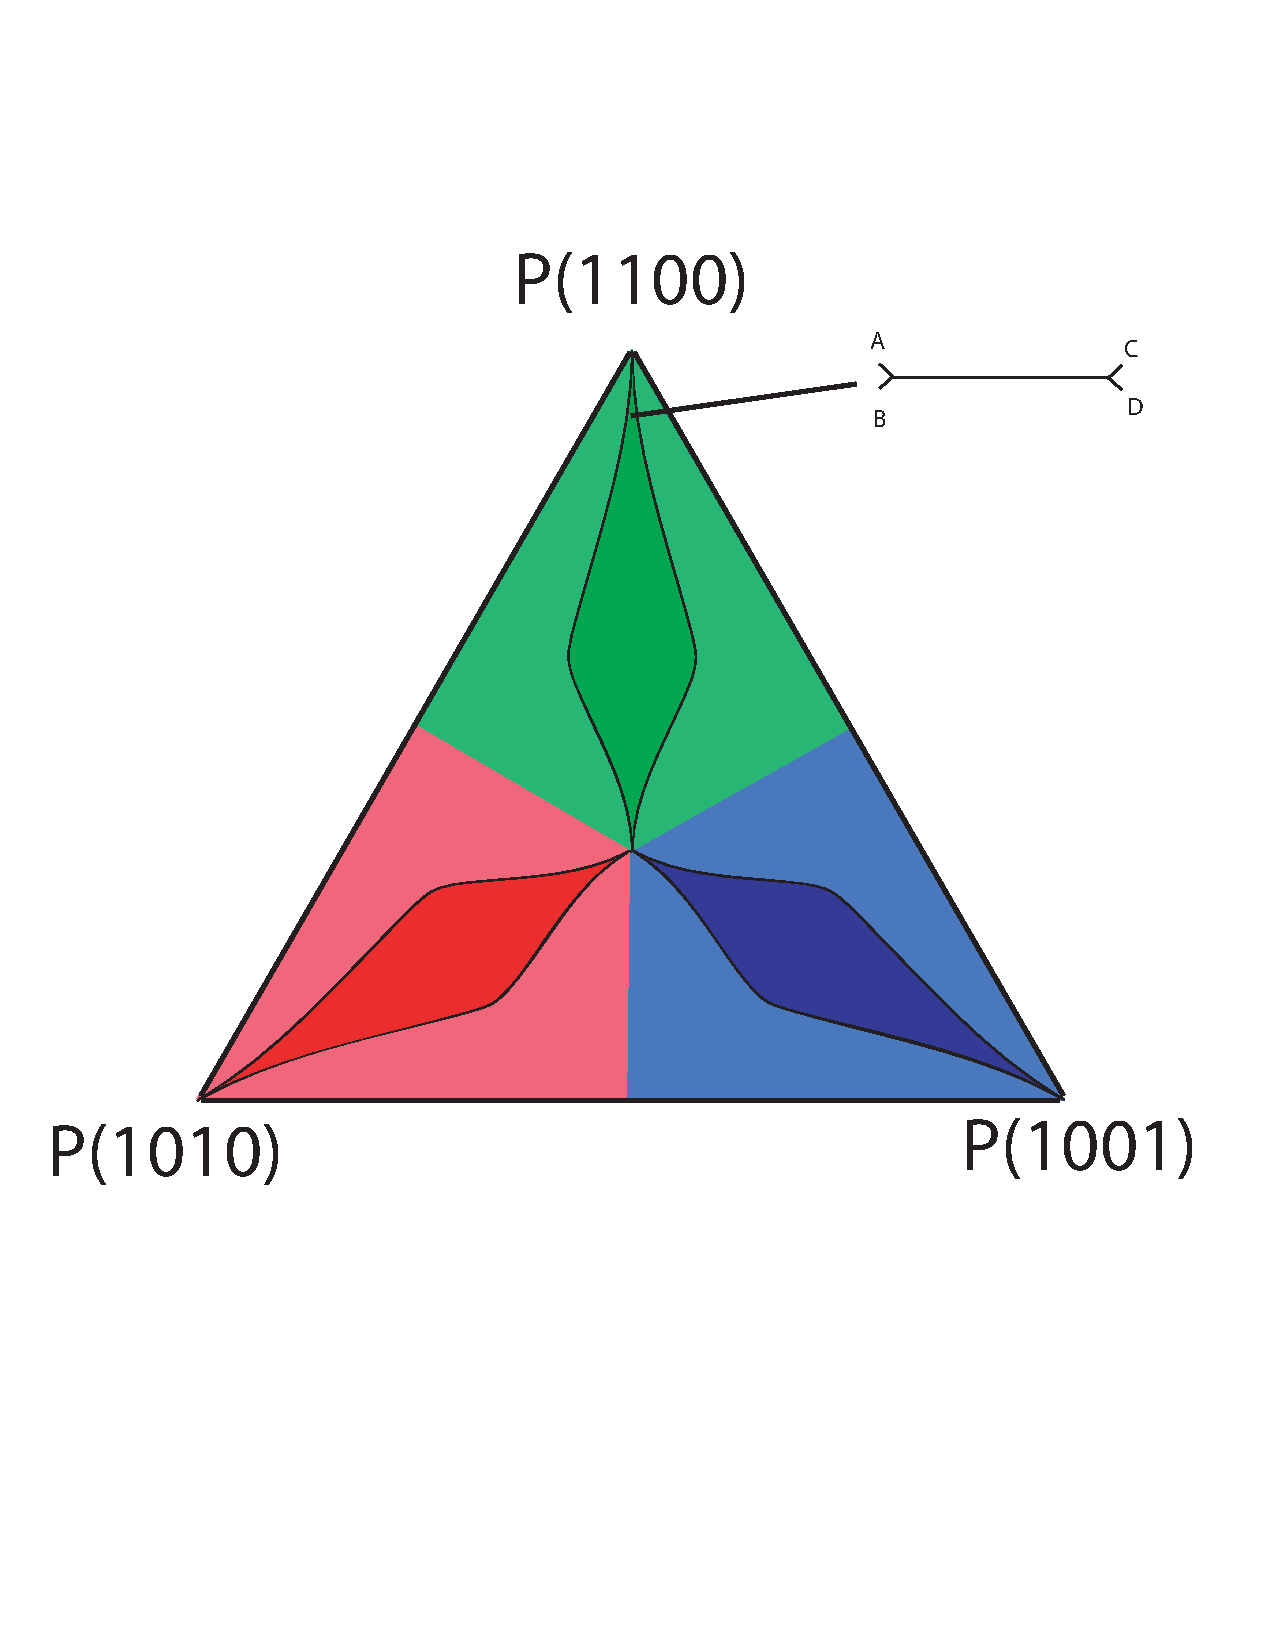
\includegraphics[scale=1.]{../newimages/simple-treespace-clean.pdf}}}
\end{picture}

\myNewSlide
\section*{Parsimony-informative Pattern Frequency Space}
\begin{picture}(-0,0)(-0,0)
	\put(10,-140){\makebox(30,-150)[l]{\includegraphics[scale=1.]{../newimages/simple-treespace-messy.pdf}}}
\end{picture}
\myNewSlide
\section*{Parsimony-informative Pattern Frequency Space}
\begin{picture}(-0,0)(-0,0)
	\put(10,-140){\makebox(30,-150)[l]{\includegraphics[scale=1.]{../newimages/simple-treespace-lba.pdf}}}
\end{picture}

\myNewSlide
\section*{Pattern Frequency Space With Observed Data}
\begin{picture}(-0,0)(-0,0)
	\put(10,-140){\makebox(30,-150)[l]{\includegraphics[scale=1.]{../newimages/simple-treespace-sample.pdf}}}
	\put(370,-183){$f_X$}
\end{picture}

\myNewSlide
\section*{ML scores in Pattern Frequency Space}
\begin{picture}(-0,0)(-0,0)
	\put(10,-120){\makebox(30,-190)[l]{\includegraphics[scale=1.]{../newimages/simple-treespace-pp1v2.pdf}}}
	\put(-30,-0){$\ln L(T_1 \mid X) = -D_{KL}(f_X \mid f_{T_1})$}
\end{picture}

\myNewSlide
\section*{LR statistics in Pattern Frequency Space}
\begin{picture}(-0,0)(-0,0)
	\put(10,-120){\makebox(30,-190)[l]{\includegraphics[scale=1.]{../newimages/simple-treespace-ppv2.pdf}}}
	\put(-50,-0){Black is the $\ln L$ between}
	\put(-50,-30){tree $AB|CD$  and tree $AC|BD$}
	\put(370,-0){Yellow is the $\ln L$ between}
	\put(380,-30){tree $AB|CD$  and tree $AD|BC$}
	
\end{picture}



\myNewSlide
\section*{aLRT and aBayes in Pattern Frequency Space}
\begin{picture}(-0,0)(-0,0)
	\put(10,-120){\makebox(30,-190)[l]{\includegraphics[scale=1.]{../newimages/simple-treespace-ppv2.pdf}}}
	\put(-50,-0){In aLRT, we use mixtures of $\chi^2$}
	\put(-40,-30){and selection bias corrections}
	\put(-40,-60){to calculate the $P$-value.}
	\put(370,-0){In aBayes, we normalize}
	\put(380,-30){the ML scores to sum to 1}
\end{picture}

\myNewSlide
\section*{Non-parametric Bootstrapping in Pattern Frequency Space}
\begin{picture}(-0,0)(-0,0)
	\put(10,-150){\makebox(30,-150)[l]{\includegraphics[scale=1.]{/home/mholder/Documents/ku_teaching/BIOL-848-2013/images/simple-treespace-boot.pdf}}}
\end{picture}

\myNewSlide
\section*{Bootstrapping in Pattern Frequency Space (if you had more data)}
\begin{picture}(-0,0)(-0,0)
	\put(-50,-0){AU Test uses multiple sequence}
	\put(-40,-30){lengths to correct BP for}
	\put(-40,-60){any curvature in the boundary }
	\put(-40,-90){between trees}
	\put(10,-150){\makebox(30,-150)[l]{\includegraphics[scale=1.]{../newimages/simple-treespace-boot-more.pdf}}}
\end{picture}

\myNewSlide
\section*{Parametric bootstrapping in Pattern Frequency Space}
\begin{picture}(-0,0)(-0,0)
	\put(10,-120){\makebox(30,-190)[l]{\includegraphics[scale=1.]{../newimages/simple-treespace-parametricBP.pdf}}}
	\put(-50,-0){Uses the $\delta$ test statistic}
	\put(-40,-30){and a null distribution}
	\put(-40,-60){{\em centered} on point that}
	\put(-40,-90){arises from the best}
	\put(-40,-120){tree in $H_0$}
\end{picture}

\myNewSlide
\section*{KH Test in Pattern Frequency Space}
\begin{picture}(-0,0)(-0,0)
	\put(10,-120){\makebox(30,-190)[l]{\includegraphics[scale=1.]{../newimages/simple-treespace-kh.pdf}}}
	\put(-50,-0){Uses the $\delta$ test statistic}
	\put(-40,-30){and a null distribution}
	\put(-40,-60){{\em centered} on the boundary}
\end{picture}


\myNewSlide
\section*{aBP in Pattern Frequency Space}
\begin{picture}(-0,0)(-0,0)
	\put(-50,-0){Null distribution for BP}
	\put(-40,-30){is calculated using}
	\put(-40,-60){Normal approximations from}
	\put(-40,-90){polytomy}
	\put(10,-150){\makebox(30,-150)[l]{\includegraphics[scale=1.]{../newimages/simple-treespace-abp.pdf}}}
\end{picture}

\myNewSlide
\section*{Summary - Part 2}
\normalsize
A (very) wide variety of tests differ by:
\begin{itemize}
	\item Null hypotheses:
	\begin{compactitem}
		\item Expected scores are the same $\rightarrow$ boundary tests. {\bf Non-parametric tests}
		\item A tree consistent with the null is correct $\rightarrow$ tests that use the full info of the model. {\bf Parametric tests}
	\end{compactitem}
	\item How to use variance information:
	\begin{compactitem}
		\item Rely on ``raw'' bootstrap variability,
		\item Invoke assumptions of normality of scores,
		\item Use $\chi^2$ variants.
	\end{compactitem}
	\item Whether or not the trees must be specified {\em a priori} -- KH Test requires the trees to be specified {\em a priori}.
\end{itemize}

\myNewSlide
\section*{Summary - Part 3}
\large
\begin{table}[htdp]
\begin{center}
\begin{tabular}{|c|p{7cm}|p{6cm}|}
\hline
& Parametric & Nonparametric \\
\hline
$P$-value from $\delta$  & aLRT, aBayes, parametric bootstrapping & KH, SH \\
\hline
$P$-value from BP  &aBP(semi)  & BP, aBP(semi), AU, EHH\\
\hline
\end{tabular}
\end{center}
\label{default}
\end{table}%

When you use a parametric test, you will usually gain power. But non-parametric tests are more robust to model violation.






\myNewSlide
\normalsize
\bibliography{phylo}

\myNewSlide
\section*{Bootstrapping as a noisy measure of repeatability}
\begin{picture}(0,0)(0,0)
	  \put(40,-280){\makebox(0,0)[l]{\includegraphics[scale=1.2]{../newimages/HillisB1993Fig3.pdf}}}
	  \put(150,-330){\small \% recovering tree}
	  \put(0,-20){\small bootstrap}
	  \put(0,-50){\small values from}
	  \put(0,-80){\small many simulations}
	  \put(0,-220){\small repeated}
	  \put(0,-250){\small simulation}
	  \put(390,-170){Simulation study of }
	  \put(390,-200){\citet{HillisB1993} }
\end{picture}


\myNewSlide
\section*{Bootstrap Proportion $\neq$ Posterior Probability}
Several studies have compared the non-parametric bootstrap proportion of clade from an ML analysis of a data set to the posterior probabilities when the same data is analyzed under the same model \citep{SuzukiGN2002,WilcoxZHH2002,AlfaroZL2003,CummingsHMRRW2003,DouadyDBDD2003}.\par

Note: {\em \bf Not} all of these have implied that the measures {\em\bf should} be the same, but some authors have \citep[usually citing][]{EfronHH1996}.

\myNewSlide
\section*{Bootstrap Proportion $\neq$ Posterior Probability in general}
\begin{picture}(-0,0)(-0,0)
	\put(40,-50){\makebox(30,-150)[l]{\includegraphics[scale=2]{/home/mholder/Documents/ku_teaching/BIOL-848-2013/images/WilcoxZHH-figure.pdf}}}
	\put(40,-330){from \citet{WilcoxZHH2002}}
	\put(40,-380){\normalsize Note: \citet{HuelsenbeckR2004} showed that the Bayesian posterior probabilities}
	\put(40,-400){\normalsize are right on the equality line, if you  simulate from the prior.}
\end{picture}


\myNewSlide
\section*{\citet{Newton1996} showed that, when you look at the median, the BP may not be biased downward}
\begin{picture}(-0,0)(-0,0)
	\put(40,-50){\makebox(30,-150)[l]{\includegraphics[scale=2]{../newimages/Newton1996Fig4.pdf}}}
	\put(40,-330){Figure 4 from \citet{Newton1996}}
\end{picture}

\myNewSlide
\section*{What did \citet{EfronHH1996} say?}
\normalsize
We can use a Bayesian model to show that $\tilde{\alpha}$ is a reasonable 
assessment of the probability that $\mathscr{R}_1$ contains $ \mu$.
Suppose we believe \textit{a priori} that $\mu$ could lie anywhere in the plane with 
equal probability. 
Then having observed $\hat{\mu}$, the \textit{a posteriori} 
distribution of  $\mu$ given  $\hat{\mu}$ is $N_2( \hat{\mu},I)$ exactly the same as the 
bootstrap distribution of $\hat{\mu}^{\ast}$. 
In other words, $\tilde{\alpha}$ is the  \textit{a posteriori}
probability of the event $\mu \in \mathscr{R}_1$, if we begin with an ``uninformative'' prior density for $\mu$.
\begin{picture}(-0,0)(-0,0)
	\put(0,-120){\makebox(30,-150)[l]{\includegraphics[scale=4]{/home/mholder/Documents/ku_teaching/BIOL-848-2013/images/EfronHH-straight-fig.pdf}}}
\end{picture}

\myNewSlide
\section*{\citet{EfronHH1996} view of tree space}
\begin{picture}(-0,0)(-0,0)
	\put(-10,-90){\makebox(30,-150)[l]{\includegraphics[scale=3]{/home/mholder/Documents/ku_teaching/BIOL-848-2013/images/EfronHH-treespace-fig.pdf}}}
\end{picture}



\myNewSlide
\section*{What did \citet{EfronHH1996} say (and mean)?}
\begin{itemize}
	\item the ``uninformative'' prior density is a uniform prior over all of pattern frequency space
	\item this is {\em not} equivalent to a prior that would be expected to yield a phylogeny (it is actually identical to the prior you would get if you assumed that all pairwise distances between taxa were $\infty$),
	\item  \citet{EfronHH1996}  were {\em not} predicting that the bootstrap proportions should be identical to those from a Bayesian phylogenetic analysis with real phylogenetic priors.
	\item  \cite{SvennbladEOB2006} have a nice paper on this subject.
\end{itemize}


\myNewSlide
\section*{\citet{Newton1996} provides an intuition for why the mean BP may be lower than repeatability}
\begin{picture}(-0,0)(-0,0)
	\put(40,-50){\makebox(30,-150)[l]{\includegraphics[scale=2]{../newimages/Newton1996Fig3.pdf}}}
	\put(40,-320){Darker ovals indicate probability contours for datasets given the truth}
	\put(60,-350){(note that repeatability $\approx$ 100\%)}
	\put(40,-380){Lighter ovals show probability contours for bootstrapping for one dataset.}
	\put(60,-410){Many real datasets will have BP much $<$ 100\%}
	\put(-40,-50){Figure 3 from \citet{Newton1996}}
\end{picture}



\includepdf[pages={28-45}]{/home/mholder/Documents/ku_teaching/BIOL-848-2013/lec16-Bootstrapping/lec16Bootstrapping.pdf} 

\includepdf[pages={6-20}]{/home/mholder/Documents/storage/talks/bodega/HolderSotU.pdf} 

\includepdf[pages={26-27}]{/home/mholder/Documents/storage/talks/bodega/HolderSotU.pdf} 

\end{document}

